\documentclass[a4paper, 12pt, twoside]{report}  
\usepackage{geometry}

% Specify required margin widths.
\geometry{
 a4paper,
 left=1.25in,
 right=1in,
 top=1in,
 bottom=1in
 }

% Specify a list of required packages.
\usepackage{graphicx}
\usepackage{fancyhdr}
\usepackage{amsmath}
\usepackage{amssymb}
\usepackage{authblk}
\usepackage{float}
\usepackage{booktabs}
\usepackage{pdfpages}
\usepackage{listings}
\usepackage{color}
\usepackage{titlesec}
\usepackage{url}
\newcommand{\apjs}{ApJS}
\newcommand{\nat}{Nature}
\newcommand{\aap}{Astronomy and Astrophysics}

% Use this package for the 'Times New Roman' font.
\usepackage{mathptmx}

% Set path/directory where all figures are stored.
\graphicspath{ {figures/} }

% Set required line spacing.
% A factor of 1.3 corresponds to 1.5 line spacing.
\linespread{1.3}

\begin{document}

\date{}

% Use '\thispagestyle{empty}' to ensure that this page
% is not counted in page numbering.
\thispagestyle{empty}

% Set required margin widths for first few pages.
\newgeometry{top = 2.5in, left = 1.25in, right = 1in, bottom = 1in}
\begin{titlepage}

    \begin{center}
        \LARGE
        \textbf{EES405- Climate Data Analysis and Visualisation}

        \vspace{1cm}


        \vspace{0.75cm}
        \Large
        \textbf{Shiv Shankar Singh}
        \vspace{1cm}

        \large
        \textit{Past and Future changes of TX10p (Cold Days) over India in General Circulation Model}

        \vspace{2cm}

        
\includegraphics[width=6cm]{HighResolutionLogo.jpg}

        \vspace{1cm}

        \large
        \textbf{Indian Institute of Science Education and Research, Mohali}\\
        \vspace{0.5cm}
        \large
        \textbf{April 2023}
    \end{center}


\end{titlepage}

% Use '\thispagestyle{empty}' to ensure that this page
% is not counted in page numbering.
\thispagestyle{empty}
\cleardoublepage

% Use Roman Page Numbering for first few pages.
\pagenumbering{Roman}



\cleardoublepage

% % Acknowledgements.
% \begin{center}
%     \textbf{\Large Acknowledgements}
% \end{center}
% I would like to express my sincere gratitude to Dr. Raju Attada, Faculty, Department of Earth and Environmental Sciences, for providing me with the opportunity to learn and visualize various temperature extremes using data science tools. This experience has helped me develop my research skills and data science skills in handling big data.

% I would also like to thank the teaching assistants for their support in answering my doubts and providing me with the shapefile for analysis. Their guidance and assistance were instrumental in helping me complete this project.

% Once again, I extend my sincere appreciation to Dr. Raju Attada and the teaching assistants for their invaluable support throughout this project.

\newpage
% Abstract of the Thesis
\addcontentsline{toc}{chapter}{\textbf{Abstract}}
\begin{center}
    \textbf{\Large Abstract}
\end{center}
Extreme cold events have a significant impact on human health, agriculture, and natural ecosystems. The tx10p index, developed by the Expert Team on Climate Change Detection and Indices (ETCCDI), measures the frequency of such events. Global warming due to anthropogenic greenhouse gas emissions has led to an increase in global temperatures, which in turn has affected various weather and climate-related events, including extreme cold and hot temperatures. Studying the trend in the tx10p index over different epochs can provide insights into the impact of global warming on extreme cold events in different regions of India  \cite{https://doi.org/10.1002/2016GL067841} .

We used the tx10p index data from two different epochs, the historical period (1850-2014) and the future period (2015-2100), to investigate the trend of extreme cold events. We employed two methods, linear regression and Mann-Kendall test, to calculate the trend. Our analysis showed that the trend of cold days is decreasing over both epochs, and the decrease is more prominent in the future period. This suggests that global warming has a significant impact on extreme cold events, and we need to develop strategies to adapt to and mitigate their effects.

Our findings have important implications for policymakers, planners, and researchers who are working towards reducing greenhouse gas emissions and developing strategies to mitigate the effects of climate change. Understanding the trend in extreme cold events can help inform these efforts and guide the development of appropriate adaptation and mitigation strategies.

\newpage
\restoregeometry

% Creates a List of All Figures.
\addcontentsline{toc}{chapter}{\textbf{List of Figures}}
\listoffigures

\newpage

% Creates a List of All Tables.
\addcontentsline{toc}{chapter}{\textbf{List of Tables}}
\listoftables

% Creates a Table of Contents.
\tableofcontents

\newpage

% Use Arabic Page Numbering for the rest of the thesis.
\pagenumbering{arabic}

% Chapter 1 - Introduction.
\chapter{Introduction}\label{chap:chapter1}
%%%
% This code snippet takes care of the required  
% Equation/Figure numbering scheme.
\renewcommand\thefigure{\thechapter.\arabic{figure}}
\renewcommand{\theequation}{\thechapter.\arabic{equation}}
\setcounter{equation}{0}
\setcounter{figure}{0}
%%%

\section{Background}
The tx10p index is a measure of the frequency of extreme cold events. It is defined as the percentage of days in a year when the daily minimum temperature falls below the 10th percentile of the baseline period (1961-1990) distribution. This index was developed by the Expert Team on Climate Change Detection and Indices (ETCCDI) as part of their effort to develop climate indices that can be used to monitor and detect changes in climate extremes.

Extreme cold events have a significant impact on human health, agriculture, and natural ecosystems. They can cause hypothermia, frostbite, and respiratory problems in humans, and can damage crops and livestock. In addition, extreme cold events can disrupt ecosystems and alter the distribution and abundance of plant and animal species.

Global warming due to anthropogenic greenhouse gas emissions has led to an increase in global temperatures, which in turn has affected various weather and climate-related events, including extreme cold and hot temperatures. Studying the trend in the tx10p index over different epochs, such as the historical period (1850-2014) and future period (2015-2100), can provide insights into the impact of global warming on extreme cold events in different regions of India.

\section{Motivation}
The motivation for studying the trend in the tx10p index lies in the need to understand the impact of global warming on extreme cold events in India. Extreme cold events have a significant impact on human health, agriculture, and natural ecosystems, and can cause severe economic and social disruption.

Studying the trend in the tx10p index can provide insights into the spatial and temporal patterns of extreme cold events in different regions of India, and how they have changed over time due to global warming. This information can be useful for policymakers, planners, and researchers to develop strategies to adapt to and mitigate the effects of extreme cold events  \cite{https://doi.org/10.1002/2016GL067841} \cite{Kumar2020}  \cite{ALEXANDER20164}  \cite{Alexander2006} .

In addition, studying the trend in the tx10p index can help us better understand the relationship between global warming and extreme cold events, and how these events may change in the future as global temperatures continue to rise. This information can inform efforts to reduce greenhouse gas emissions and develop strategies to mitigate the effects of climate change.

\chapter{Data and Methods}


\section{Data}
In our study we have used the dataset from \textit{CMIP6(\textit{Coupled Model Intercomparison Project Phase 6}) }global climate model. These simulations cover a range of historical, current, and future climate scenarios, enabling researchers to investigate the impacts of climate change and potential adaptation and mitigation strategies. The CMIP6 data is available from the \textit{Earth System Grid Federation} (ESGF) and is accessible through the \textit{Climate Data Gateway} (CDG) at the National Center for Atmospheric Research (NCAR). The data is available in the \textit{NetCDF} format. The data is available for two different epochs 1850-2014 (\textit{historical}) and 2015-2100 (\textit{future projections})



\section{Methods}

\begin{enumerate}
    \item To remap and regrid data to the Indian shapefile output, we can use a combination of {\fontfamily{qcr}\selectfont xarray} ,  {\fontfamily{qcr}\selectfont rasterio} , and  {\fontfamily{qcr}\selectfont geopandas}  libraries. Here is a general outline of the steps involved:
          \begin{itemize}
              \item Load the data into an xarray dataset.
              \item Create a meshgrid of the latitude and longitude coordinates using {\fontfamily{qcr}\selectfont numpy}.
              \item
                    Load the Indian shapefile using {\fontfamily{qcr}\selectfont geopandas}.
                    Reproject the Indian shapefile to the same projection as the dataset using {\fontfamily{qcr}\selectfont pyproj}.
              \item
                    Convert the reprojected shapefile to a raster using {\fontfamily{qcr}\selectfont rasterio} .
              \item
                    Create a new dataset that has the same dimensions as the Indian shapefile raster using {\fontfamily{qcr}\selectfont xarray}.
              \item
                    Resample the original dataset to match the resolution and extent of the Indian shapefile raster using {\fontfamily{qcr}\selectfont rasterio}.
              \item
                    Apply the Indian shapefile mask to the resampled data using {\fontfamily{qcr}\selectfont numpy}.
              \item
                    Save the remapped and regridded data to a new file using {\fontfamily{qcr}\selectfont xarray}.
          \end{itemize}
    \item To calculate the trends in timeseries, we have used two different methods:
          \begin{itemize}
              \item \textbf{Linear Regression:} \\
                    The linear regression method is a statistical technique used to model the relationship between two variables by fitting a linear equation to the data. In the context of time series data, linear regression can be used to determine the trend in the data over time. The slope of the linear regression line represents the rate of change in the data over time, which can be interpreted as the trend. If the slope is positive, then the data is increasing over time, while if the slope is negative, then the data is decreasing over time. The linear regression line can be calculated using the following equation:

                    \begin{equation}
                        y = a + bx
                    \end{equation}


                    where $y$ is the dependent variable (the time series data), $x$ is the independent variable (the time), $a$ is the intercept, and $b$ is the slope. The slope of the linear regression line can be calculated using the following equation:

                    \begin{equation}
                        b = \frac{\sum_{i=1}^{n} (x_i - \bar{x})(y_i - \bar{y})}{\sum_{i=1}^{n} (x_i - \bar{x})^2}
                    \end{equation}

                    where $n$ is the number of data points, $x_i$ and $y_i$ are the $i$-th data points, $\bar{x}$ and $\bar{y}$ are the means of $x$ and $y$ respectively. The statistical significance of the slope can be calculated using the {\fontfamily{qcr}\selectfont scipy.stats}.linregress function, which returns the slope, intercept, correlation coefficient, p-value, and standard error of the slope.

              \item \textbf{Mann - Kendall Test:} \cite{pymannkendall}\\
                    The Mann-Kendall test is a non-parametric statistical test used to determine if there is a monotonic trend (i.e., a consistently increasing or decreasing pattern) in time series data. The test compares the number of increasing and decreasing values in the time series, and calculates a statistic called the Kendall tau rank correlation coefficient. If the Kendall tau coefficient is positive, then there is a monotonic increasing trend, while if it is negative, then there is a monotonic decreasing trend.

                    To perform a Mann-Kendall test on time series data, we can use the {\fontfamily{qcr}\selectfont pymannkendall} library in Python. This library provides a function called mk-test that calculates the Kendall tau coefficient and its statistical significance. \\

                    The Mann-Kendall test involves calculating the Kendall tau rank correlation coefficient ($\tau$) between the time series data ($X_i$) and its time-lagged version ($X_j$), where $j=i+1, i+2,...,n$:

                    \begin{equation}
                        \tau = \frac{2}{n(n-1)}\sum_{i=1}^{n-1}\sum_{j=i+1}^{n} \text{sign}(X_j-X_i)
                    \end{equation}

                    where $n$ is the number of data points and $\text{sign}(X_j-X_i)$ is the sign of the difference between the two data points.

                    The variance of the Kendall tau coefficient can be estimated using:
                    \begin{equation}
                        Var(\tau) = \frac{n(n-1)(2n+5)}{18}
                    \end{equation}


                    and the standard error can be calculated as:
                    \begin{equation}
                        SE(\tau) = \sqrt{Var(\tau)}
                    \end{equation}

                    The test statistic ($Z$) is then calculated as:
                    \begin{equation}
                        Z = \begin{cases}
                            \frac{\tau - 1}{SE(\tau)}, & \text{if } \tau < 0    \\
                            \frac{\tau}{SE(\tau)},     & \text{if } \tau \geq 0
                        \end{cases}
                    \end{equation}


                    The p-value can be calculated using the standard normal distribution function:
                    \begin{equation}
                        p = \begin{cases}
                            2(1-\Phi(|Z|)), & \text{if } Z < 0    \\
                            2\Phi(-|Z|),    & \text{if } Z \geq 0
                        \end{cases}
                    \end{equation}


                    where $\Phi$ is the standard normal distribution function.

                    If the p-value is less than a specified significance level (e.g., 0.05), then the null hypothesis (i.e., no trend) can be rejected, and a monotonic trend can be inferred. Otherwise, there is insufficient evidence to reject the null hypothesis.
          \end{itemize}

\end{enumerate}




\chapter{Results and Discussion}

\section{Spatial plot of climatology of TX10p for the historical period (1851-2014) over (60E-100E, 5-40N)}

\begin{figure}[htb]
    \centering
    \includegraphics[width=0.95\textwidth]{/home/shiv/Documents/GitHub/EES405/assignment_4/plots/tx10p-historical-spatial-climatology-india-shapefile.png}
    \caption{\centering Spatial plot of climatology of TX10p for the historical period (1851-2014) over (60E-100E, 5-40N)}
    \label{fig:TX10p_spatial}
\end{figure}

In the above plot , we can see the spatial plot of climatology of cold days in the historical epoch (1850-2014). The cold days climate index is calculated as the percentage of days with maximum temperature below the corresponding calendar day 10th percentile of maximum temperature for a 5-day moving window in the base period.


\section{Spatial trend of TX10p for the historical epoch (1850-2014)}

\begin{figure}[h]
    \centering
    \includegraphics[width=0.95\textwidth]{/home/shiv/Documents/GitHub/EES405/assignment_4/plots/spatial-trend-historical-india-shapefile.png}
    \caption{\centering Spatial trend of TX10p for the historical epoch (1850-2014) (Black dots are places with significant trend value)}
    \label{fig:TX10p_spatial_trend}
\end{figure}

In the above plot , we can see the spatial trend plot of TX10p for the historical epoch (1850-2014). The blue regions represent negative trends, while the red regions represent positive trends. In this context:

Positive trends (red regions) indicate that the frequency of cold days (days when the daily maximum temperature is below the 10th percentile) is increasing over time. This could be interpreted as a sign of increasing temperatures or more frequent heatwaves.
Negative trends (blue regions) indicate that the frequency of hot days is decreasing over time. This could be interpreted as a sign of decreasing temperatures or less frequent heatwaves.

\section{Area averaged (60E-100E, 5-40N) timeseries of TX10p index from 1851-2014 (Historical epoch) over different parts of the Indian region.}

Timeseries of TX10p index from 1851-2014 (Historical epoch) over
\begin{itemize}
    \item North India (72E-80E, 29-37N)
    \item Central India (75E-85E, 18-29N)
    \item West India (68E - 75E, 18E - 29.2E)
    \item East India (85E - 97.5E, 19E - 29E)
    \item South India (73E - 83E, 8E - 18E)
\end{itemize}


One can calculate the files for various regions either via \textit{CDO command -cdo sellonlatbox,lon-min, lon-max, lat-min, lat-max} or via \textit{Python slice commands} \cite{cdo}.

\subsection{North India (72E-80E, 29-37N) timeseries plot of TX10p index}

\begin{figure}[h]
    \centering
    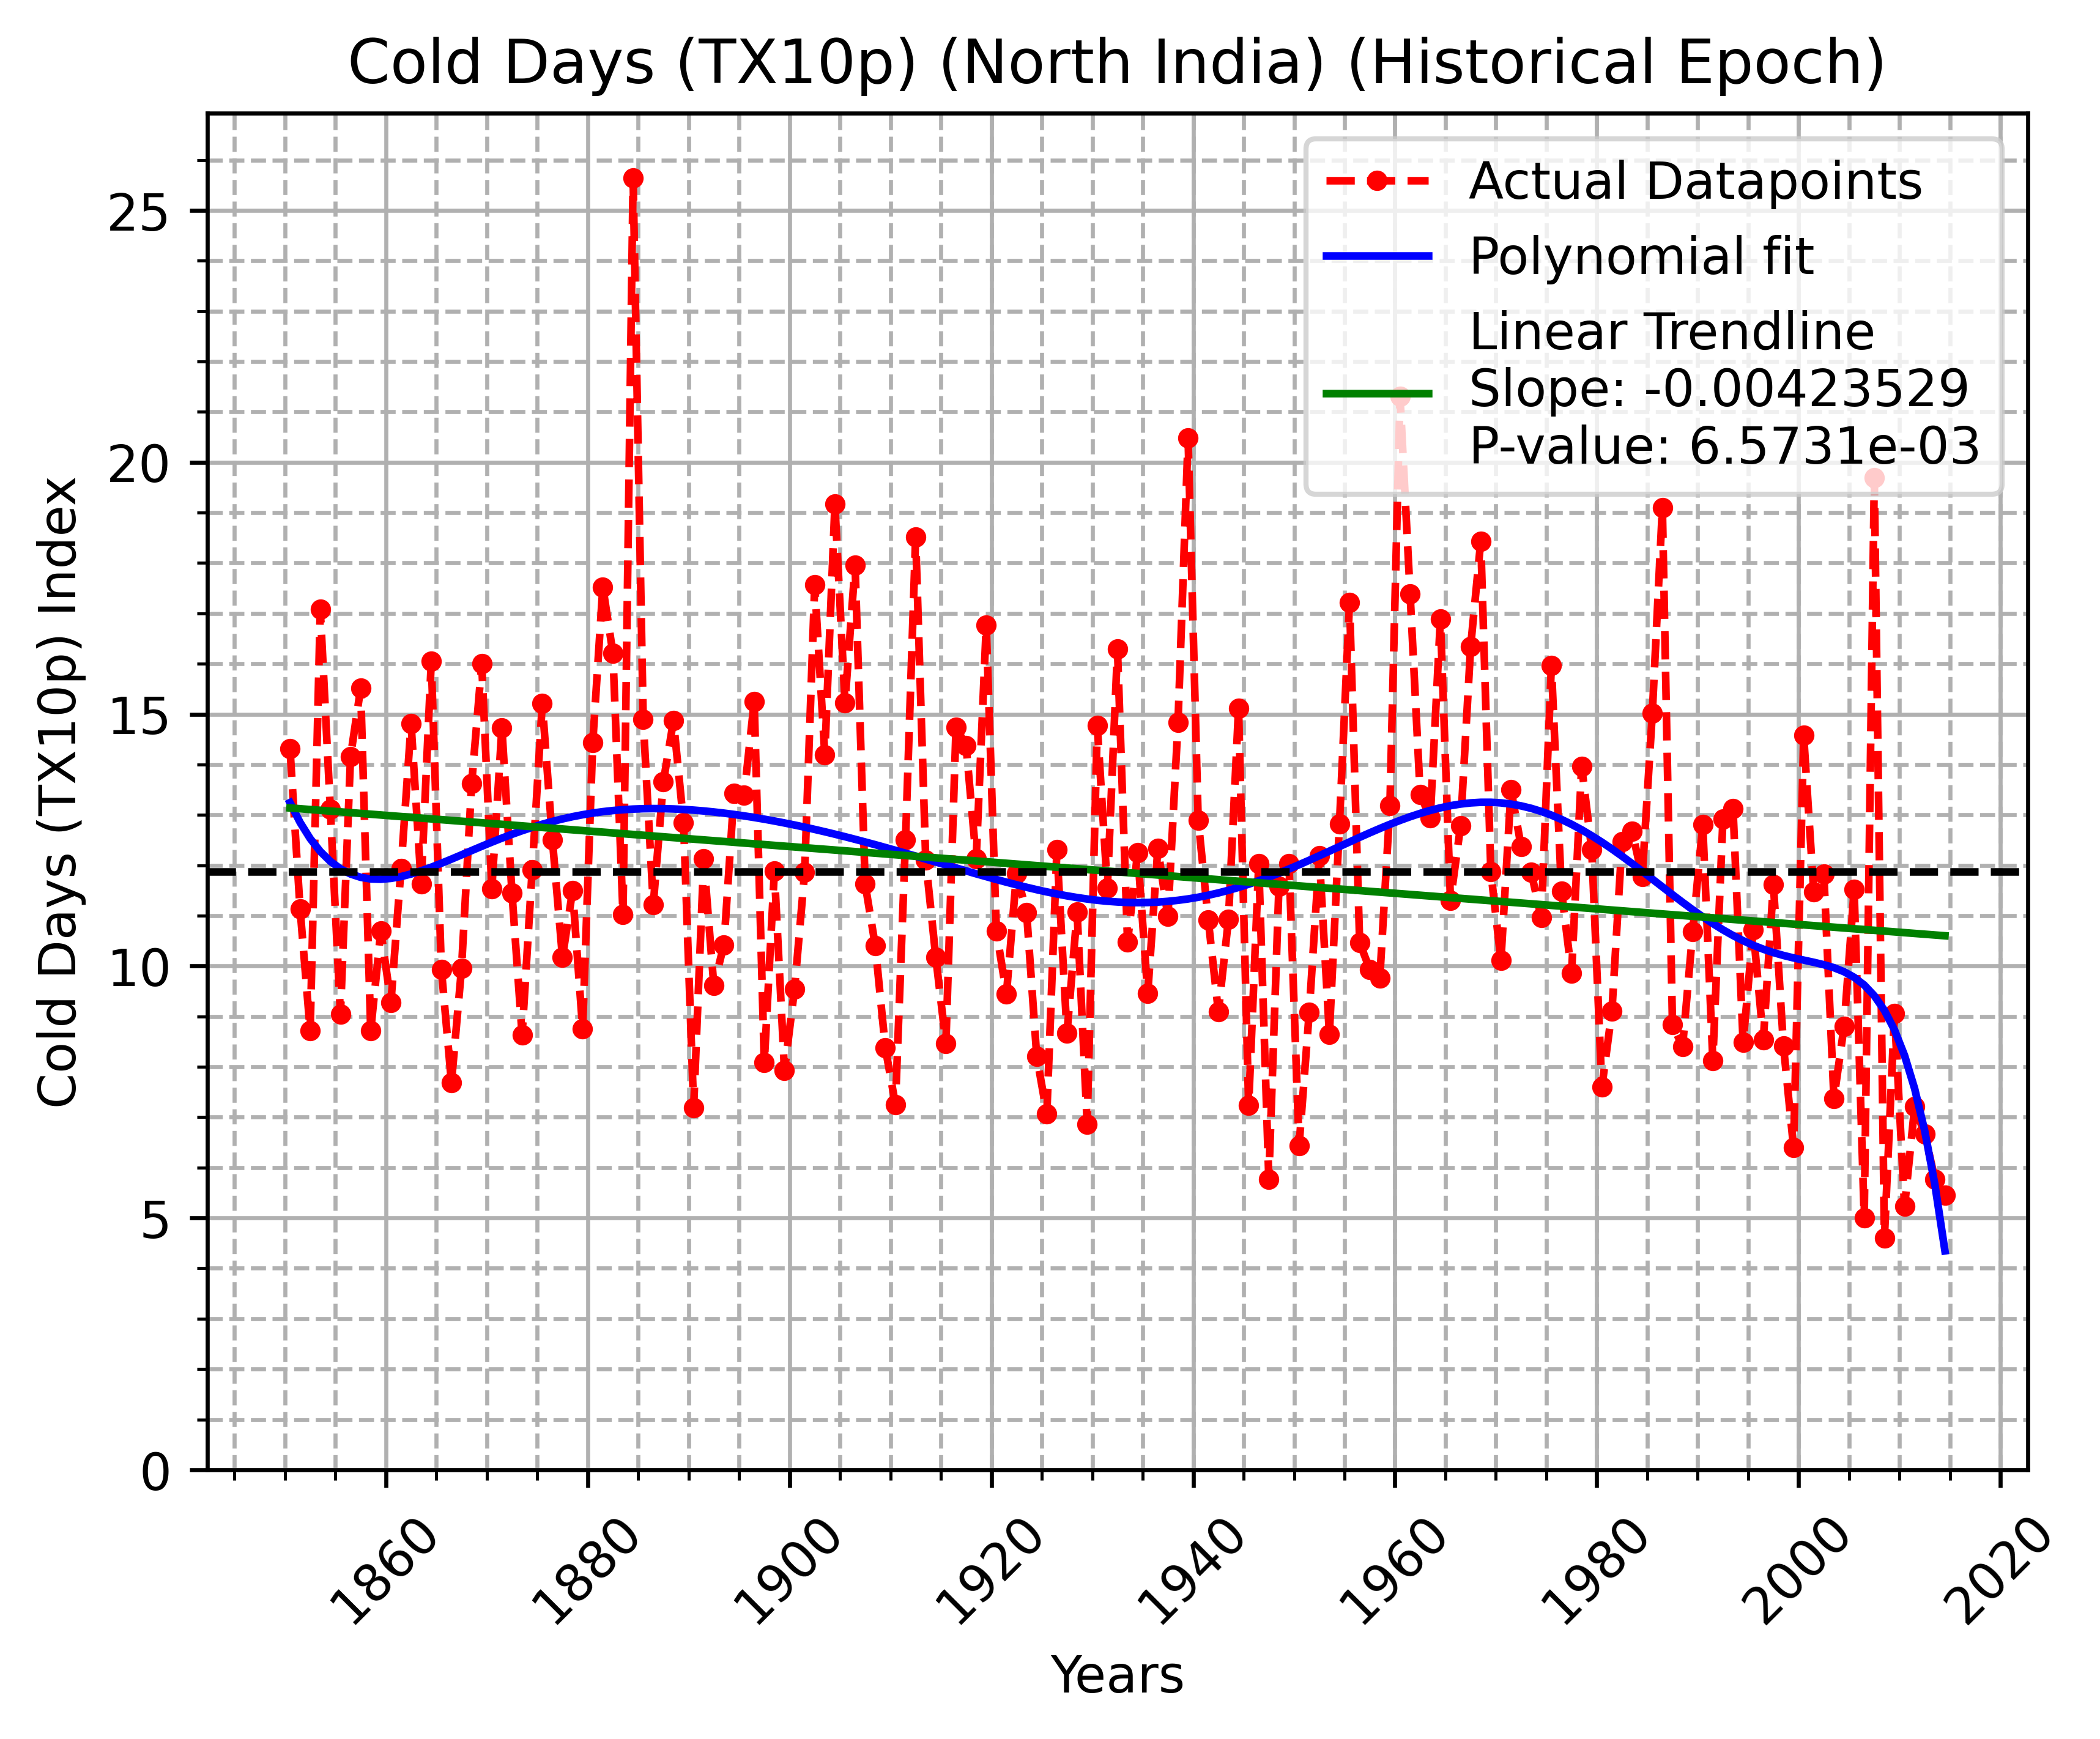
\includegraphics[width=0.95\textwidth]{/home/shiv/Documents/GitHub/EES405/assignment_4/plots/tx10p.north_india_hist.png}
    \caption{\centering Timeseries plot of TX10p index from 1851-2014 (Historical epoch) over North India (72E-80E, 29-37N)}
    \label{fig:TX10p_timeseries_north_india}
\end{figure}

From the above plot, we can infer that the frequency of cold days is decreasing over time in the North Indian region. This could be interpreted as a sign of increasing temperatures or more frequent heatwaves.



\subsection{Central India (75E-85E, 18-29N) timeseries plot of TX10p index}

\begin{figure}[h]
    \centering
    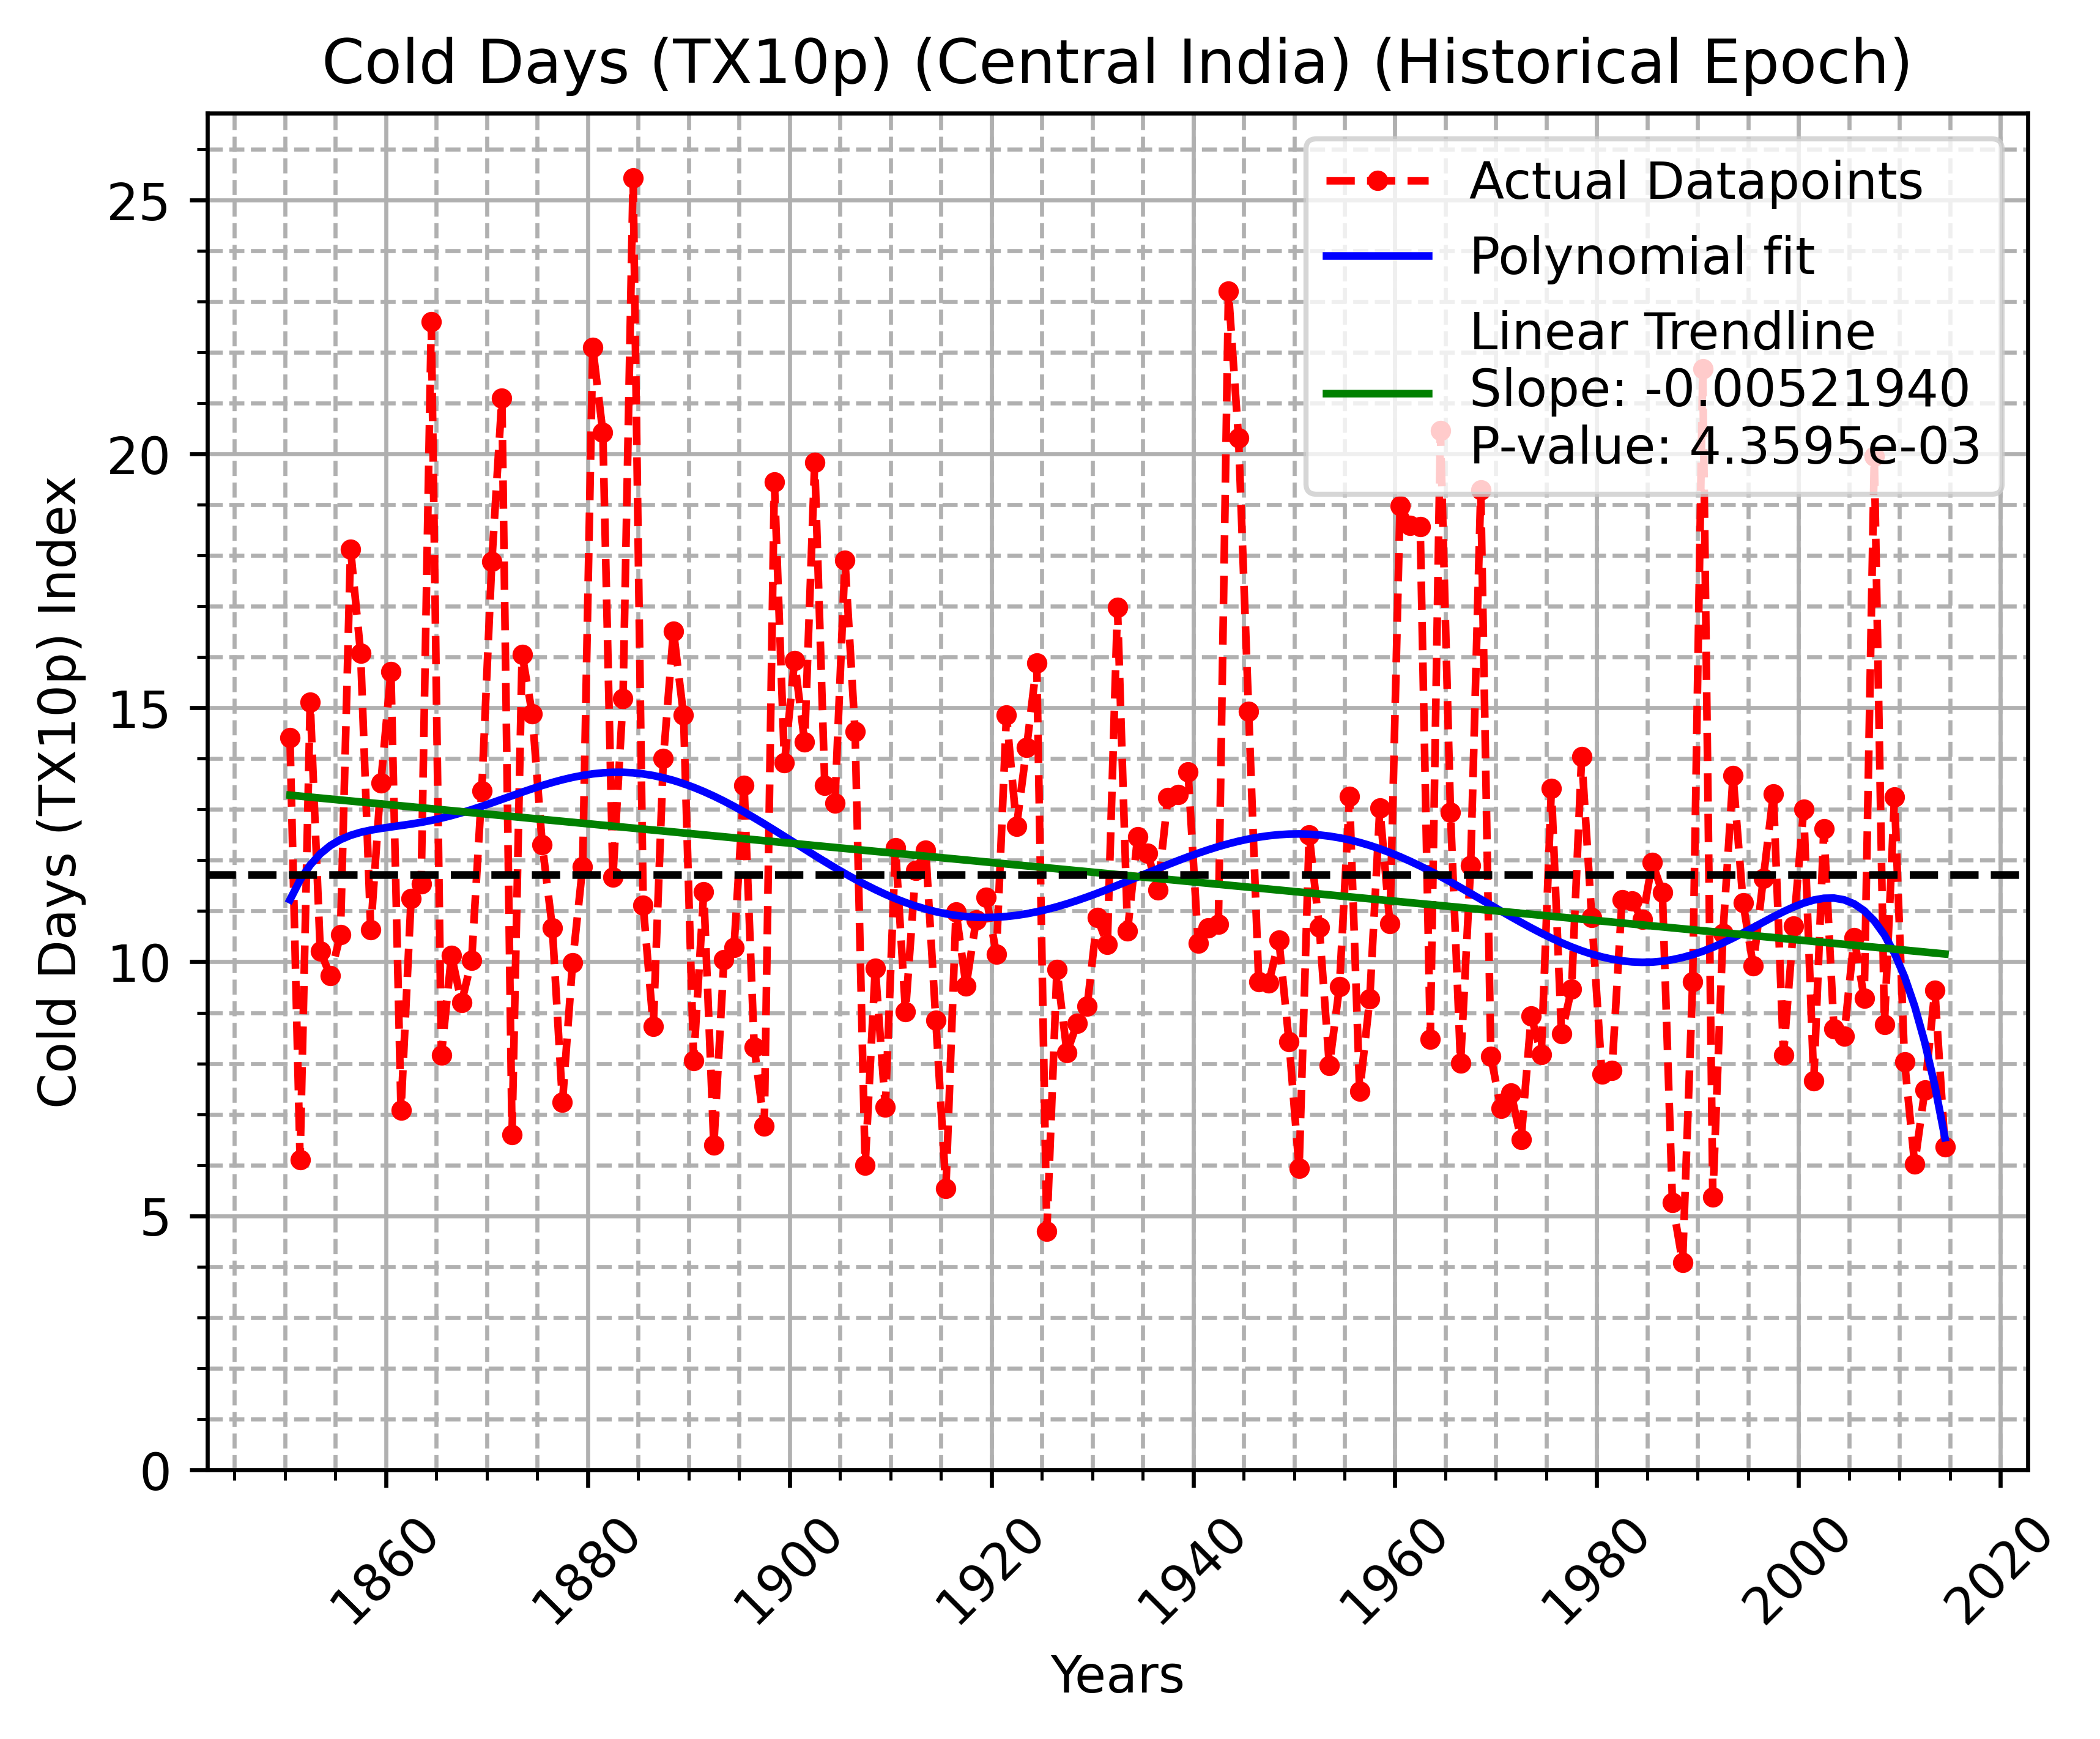
\includegraphics[width=0.95\textwidth]{/home/shiv/Documents/GitHub/EES405/assignment_4/plots/tx10p.central_india_hist.png}
    \caption{\centering Timeseries plot of TX10p index from 1851-2014 (Historical epoch) over Central India (72E-80E, 29-37N)}
    \label{fig:TX10p_timeseries_central_india}
\end{figure}

We observe a similar trend in the central Indian region as well. The frequency of cold days is decreasing over time in the central Indian region. This could be interpreted as a sign of increasing temperatures or more frequent heatwaves. This increasing temperature can be attributed to the increasing anthropogenic emissions of greenhouse gases in the atmosphere. We also observe that the decadal decrease in the percentage of cold days is more pronounced in the central Indian region than in the North Indian region. This could be attributed to the fact that the central Indian region is more densely populated than the North Indian region and hence more susceptible to the effects of climate change caused due to human influence.
\newpage
\subsection{West India (68E - 75E, 18E - 29.2E) timeseries plot of TX10p index}

\begin{figure}[h]
    \centering
    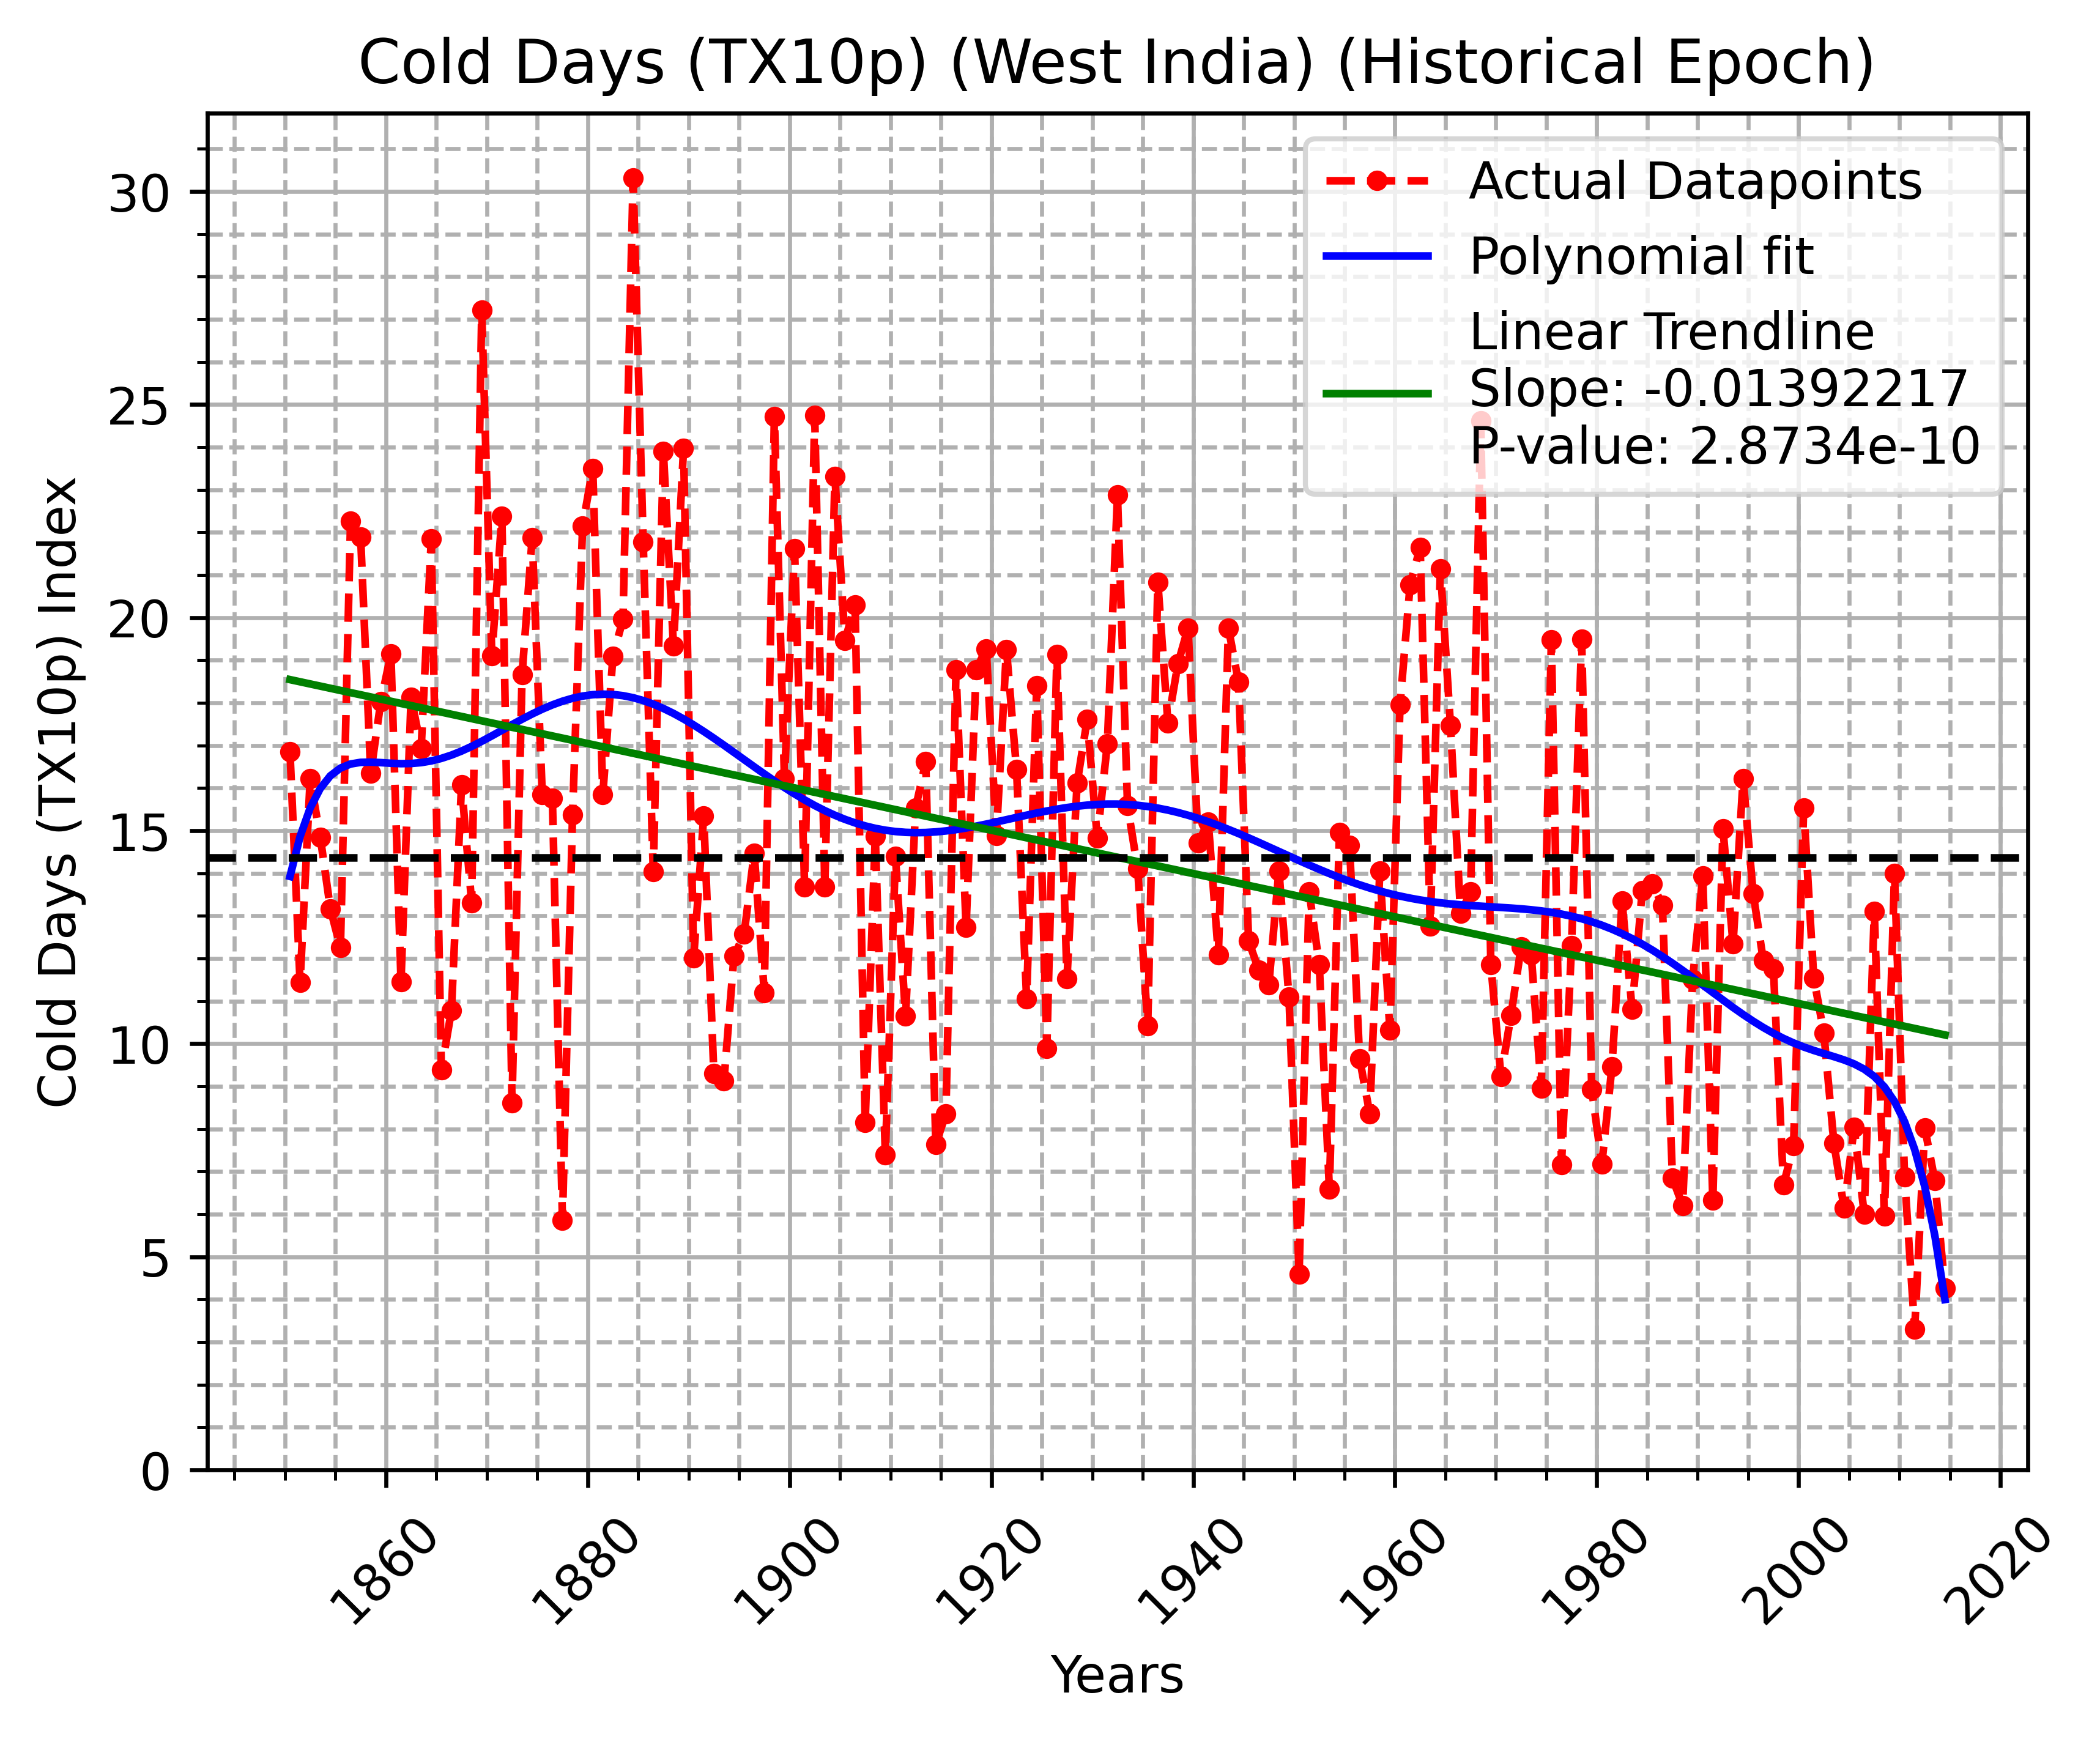
\includegraphics[width=0.95\textwidth]{/home/shiv/Documents/GitHub/EES405/assignment_4/plots/tx10p.west_india_hist.png}
    \caption{\centering Timeseries plot of TX10p index from 1851-2014 (Historical epoch) over West India (68E - 75E, 18E - 29.2E)}
    \label{fig:TX10p_timeseries_west_india}
\end{figure}

In the above plot, we see a similar trend of decreasing cold days as expected in western India as well. The frequency of cold days is decreasing over time in the western Indian region. The decadal decrease in the percentage of cold days is more pronounced than North and central Indian regions. This could be attributed to the fact that the western Indian region contains the most densely populated cities in India and hence more susceptible to the effects of climate change caused due to human influence.
\newpage
\subsection{East India (85E - 97.5E, 19E - 29E) timeseries plot of TX10p index}

\begin{figure}[h]
    \centering
    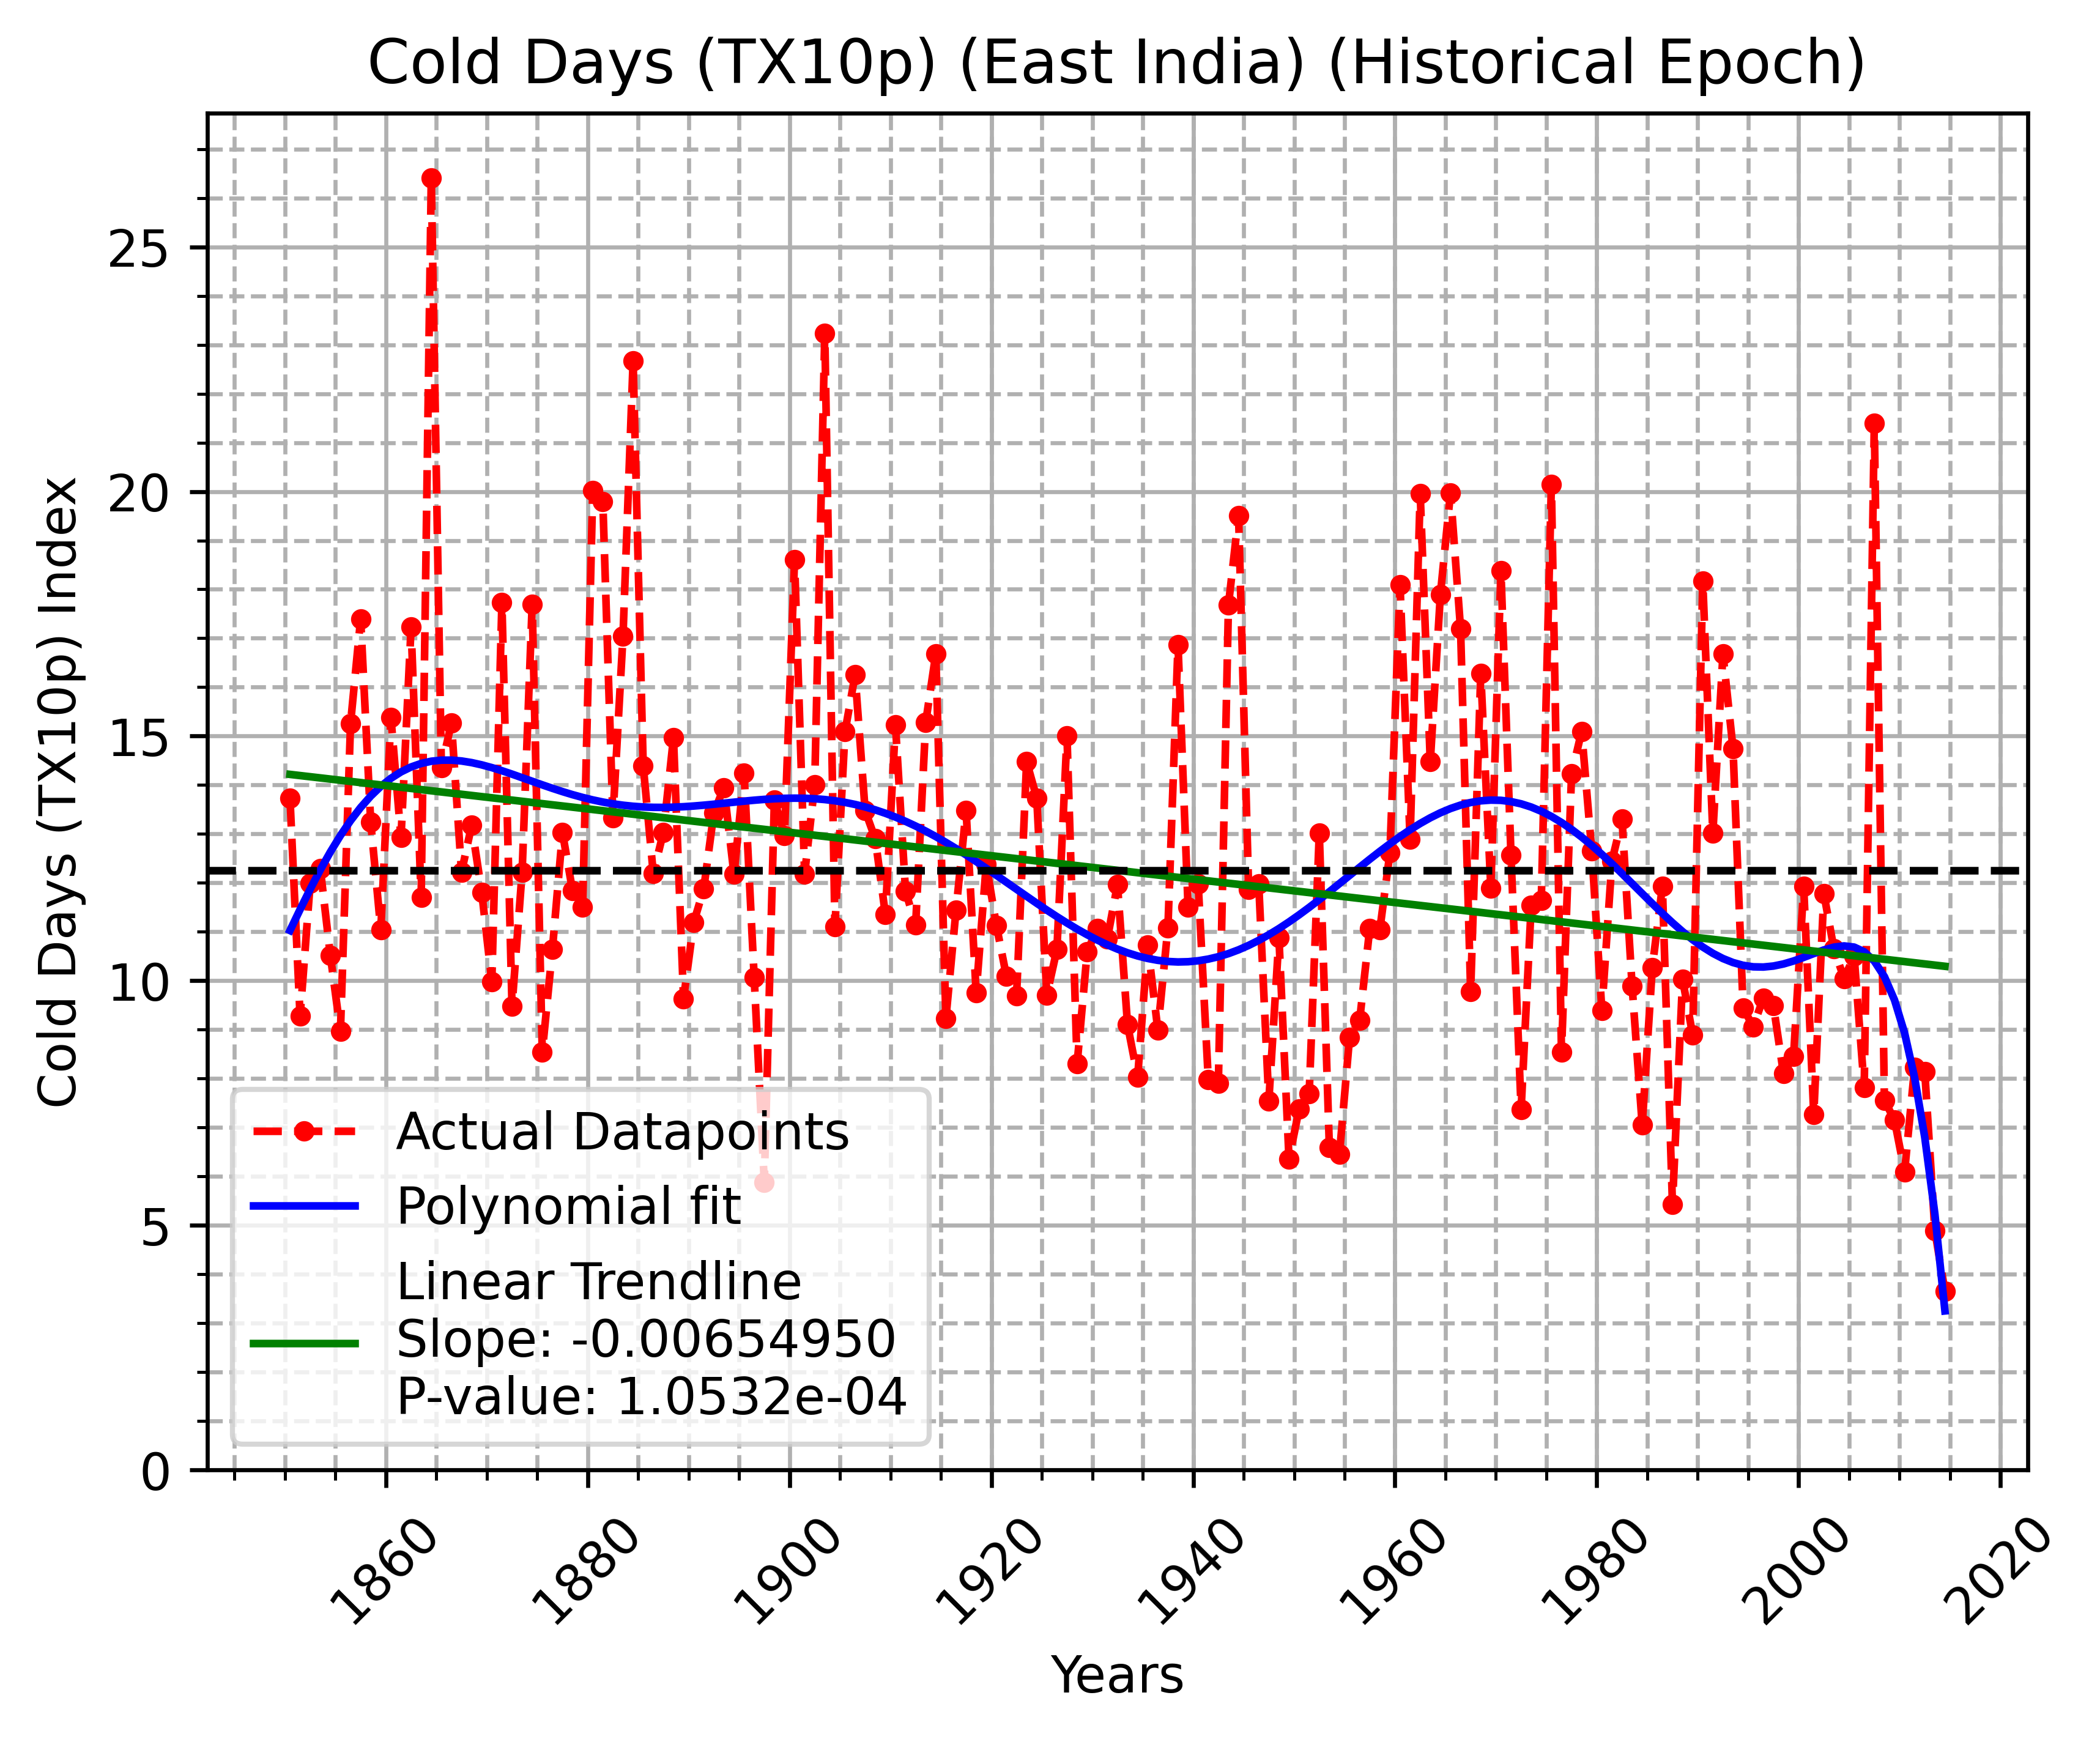
\includegraphics[width=0.95\textwidth]{/home/shiv/Documents/GitHub/EES405/assignment_4/plots/tx10p.east_india_hist.png}
    \caption{\centering Timeseries plot of TX10p index from 1851-2014 (Historical epoch) over East India (85E - 97.5E, 19E - 29E)}
    \label{fig:TX10p_timeseries_east_india}
\end{figure}

In the above plot, we see a similar trend of decreasing cold days as expected in eastern India as well. The frequency of cold days is decreasing over time in the eastern Indian region. The decadal decrease in the percentage of cold days is less pronounced than the western Indian region. This could be attributed to the fact that the eastern Indian region is less densely populated than the western Indian region and hence less susceptible to the effects of climate change caused due to human influence.

\newpage

\subsection{South India (73E - 83E, 8E - 18E) timeseries plot of TX10p index}

\begin{figure}[h]
    \centering
    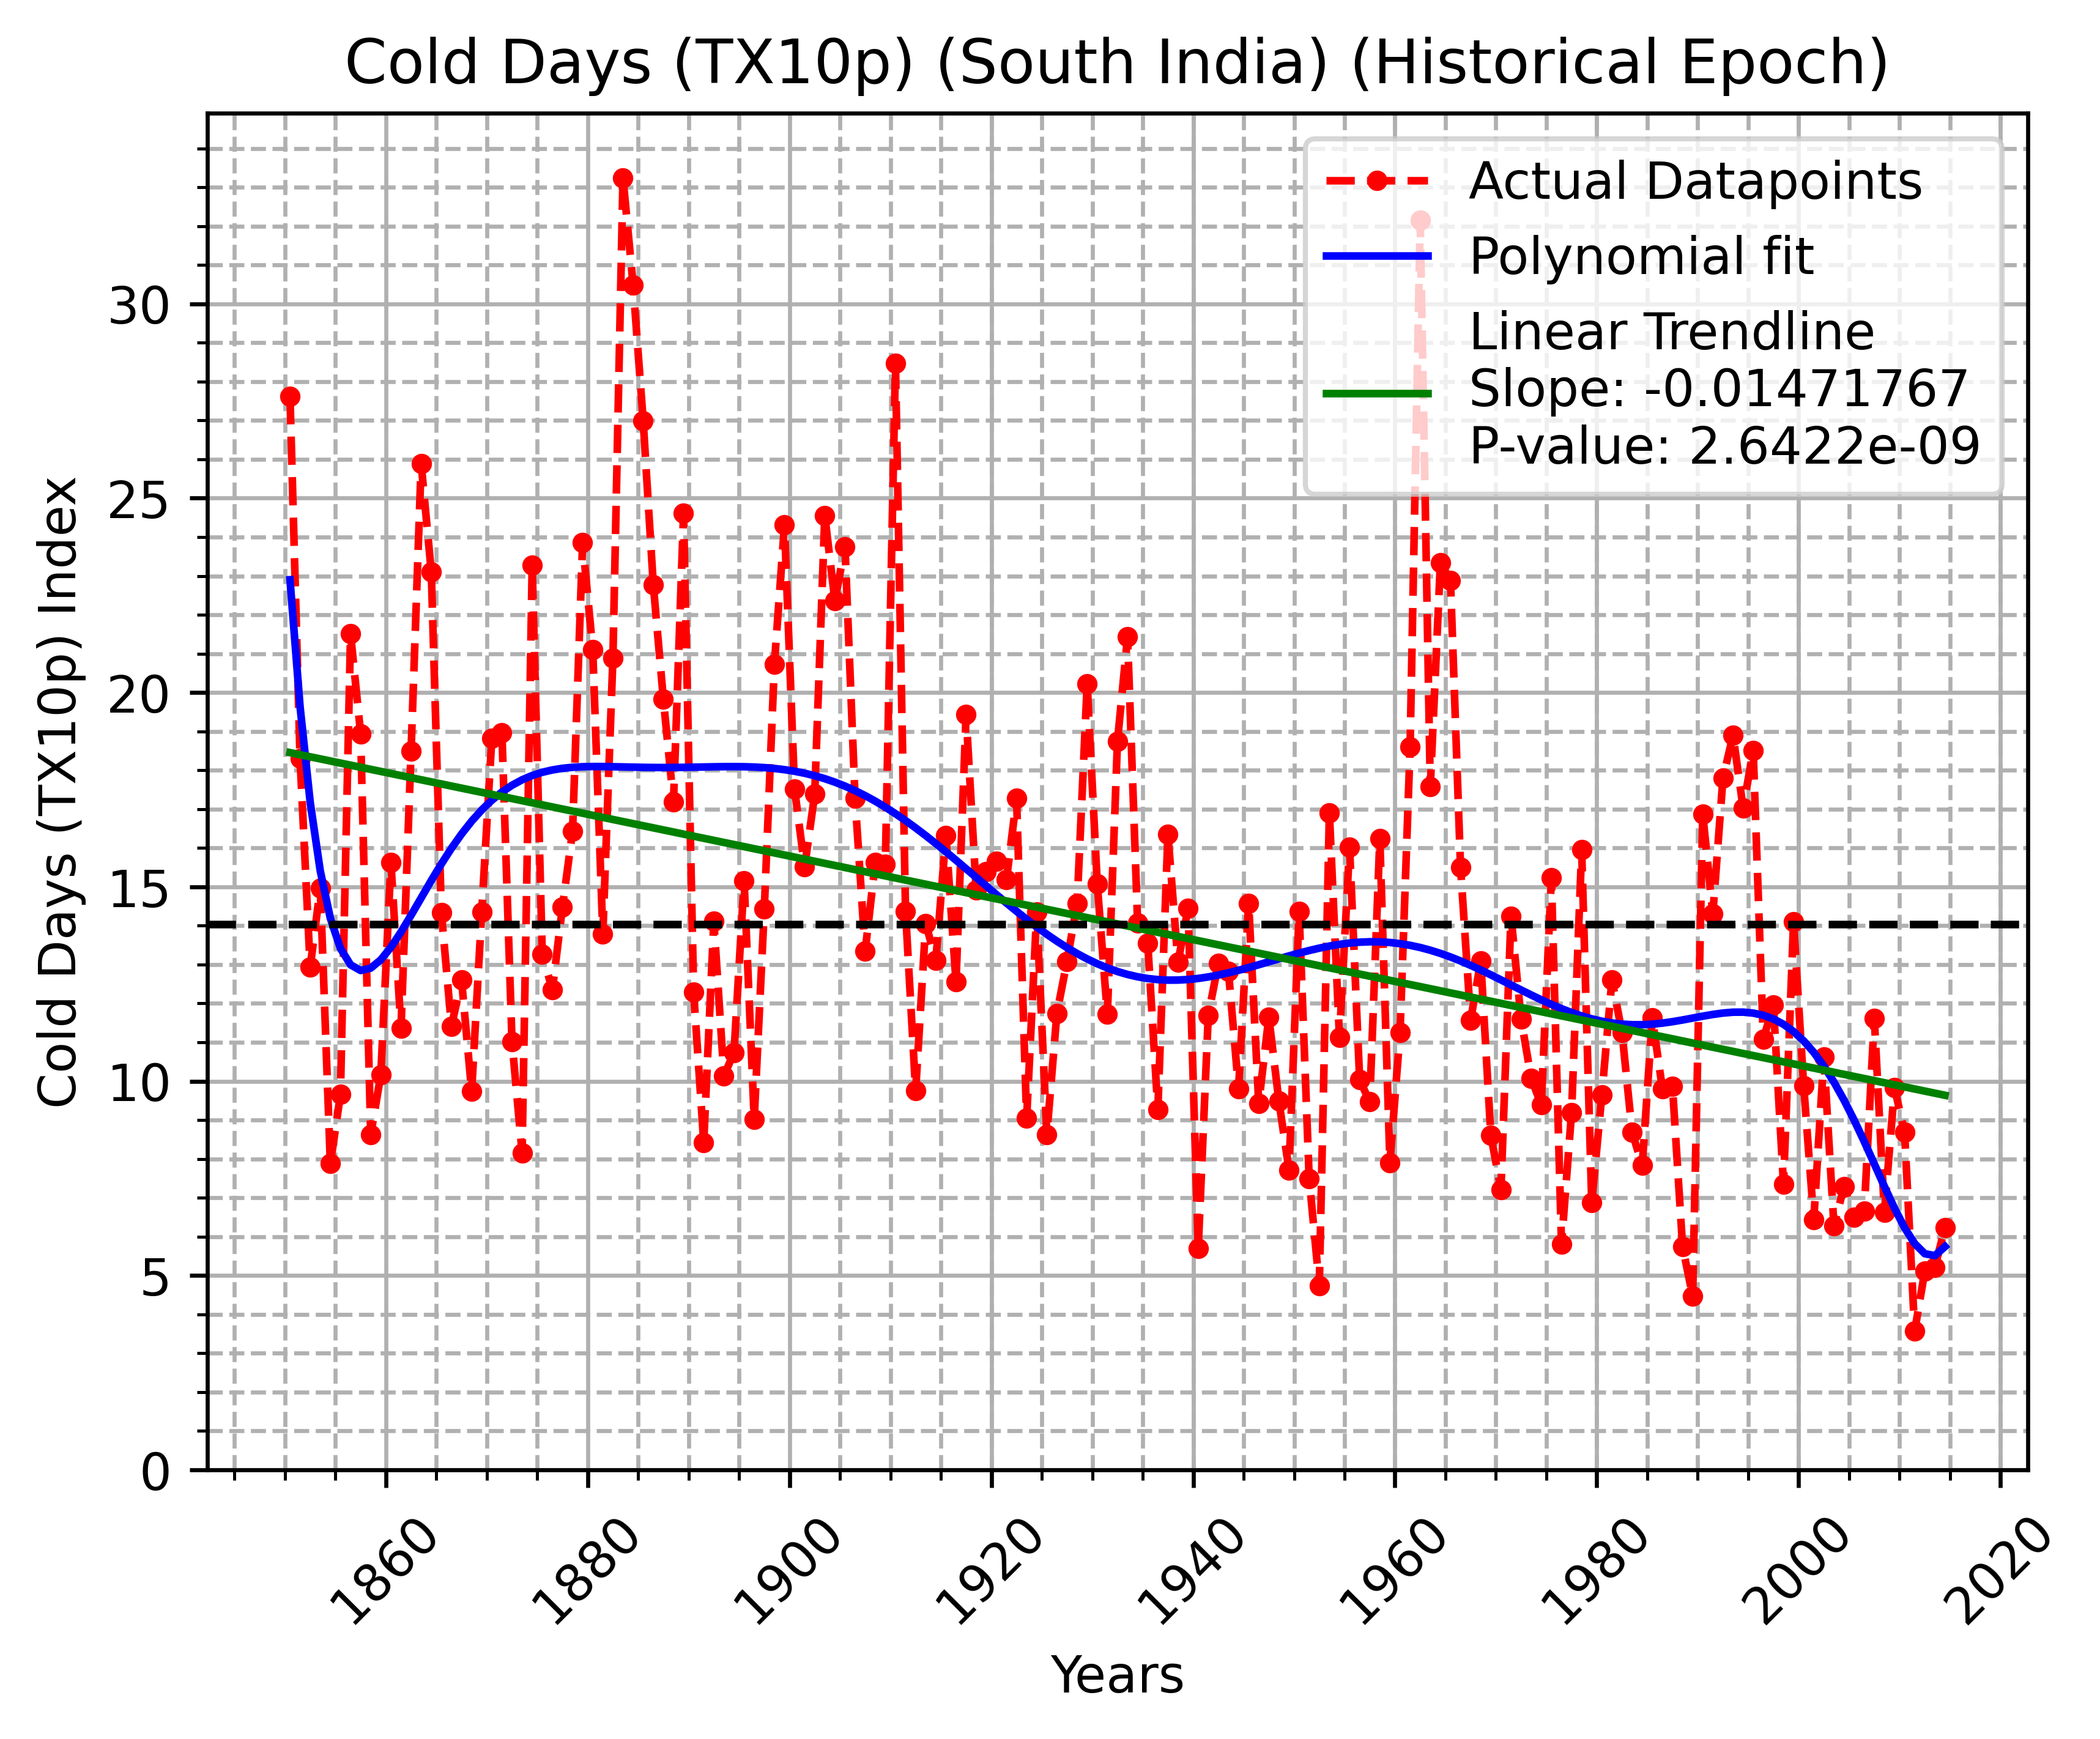
\includegraphics[width=0.95\textwidth]{/home/shiv/Documents/GitHub/EES405/assignment_4/plots/tx10p.south_india_hist.png}
    \caption{\centering Timeseries plot of TX10p index from 1851-2014 (Historical epoch) over South India (73E - 83E, 8E - 18E)}
    \label{fig:TX10p_timeseries_south_india}
\end{figure}

In the above plot, we see a similar trend of decreasing cold days as expected in southern India as well. The frequency of cold days is decreasing over time in the southern Indian region. The decadal decrease in the percentage of cold days is highest amongst all the Indian regions studied in the present work. This could be attributed to the fact that the southern Indian region is highly populated as well lies below the tropics and hence more susceptible to the effects of climate change caused due to human influence. \\
In all the above timeseries plots, we see a similar trend of decreasing cold days as expected in all the Indian regions. The frequency of cold days is decreasing over time in all the Indian regions. The decadal decrease in the percentage of cold days is more pronounced in the central and southern Indian regions than in the North and East Indian regions. This could be attributed to the fact that the central and southern Indian regions are more densely populated than the North and East Indian regions and west contains mega cities of India such as Mumbai and hence more susceptible to the effects of climate change caused due to human influence.

\section{Spatial plot of climatology of TX10p for the Future epoch (2015-2100) over (60E-100E, 5-40N)}

\begin{figure}[h]
    \centering
    \includegraphics[width=0.95\textwidth]{/home/shiv/Documents/GitHub/EES405/assignment_4/plots/tx10p-future-spatial-shapefile-nan-climatology.png}
    \caption{\centering Spatial plot of climatology of TX10p for the Future epoch (2015-2100) over (60E-100E, 5-40N)}
    \label{fig:TX10p_future}
\end{figure}

In the above plot, we see a time-averaged climatology of TX10p for the Future epoch (2015-2100) over (60E-100E, 5-40N). We observe that the climatology of TX10p has decreased in all parts of the Indian region predicting the more pronounced effect of climate change in the future.

\newpage

\section{Spatial trend of TX10p for the Future epoch (2015-2100) over (60E-100E, 5-40N)}

\begin{figure}[h]
    \centering
    \includegraphics[width=0.95\textwidth]{/home/shiv/Documents/GitHub/EES405/assignment_4/plots/spatial-trend-future-india-shapefile.png}
    \caption{\centering Spatial trend of TX10p for the Future epoch (2015-2100) over (60E-100E, 5-40N) (Black Dots are places with significant trend value)}
    \label{fig:TX10p_future_trend}
\end{figure}

In the above plot, we see the spatial trend of TX10p for the Future epoch (2015-2100) over (60E-100E, 5-40N). We observe that the trend of TX10p has decreased in all parts of the Indian region predicting the more pronounced effect of climate change in the future. We see negative trend of TX10p for the entire Indian regions predicted by the CMIP6 models. This is in agreement with the increase in anthropogenic greenhouse gases in the atmosphere which is causing the global warming and hence the decrease in the frequency of cold days in the future.
\section{Area averaged (60E-100E, 5-40N) timeseries of TX10p index from 1851-2014 (Future epoch) over different parts of the Indian region.}

\subsection{North India (72E-80E, 29-37N) timeseries plot of TX10p index}

\begin{figure}[h]
    \centering
    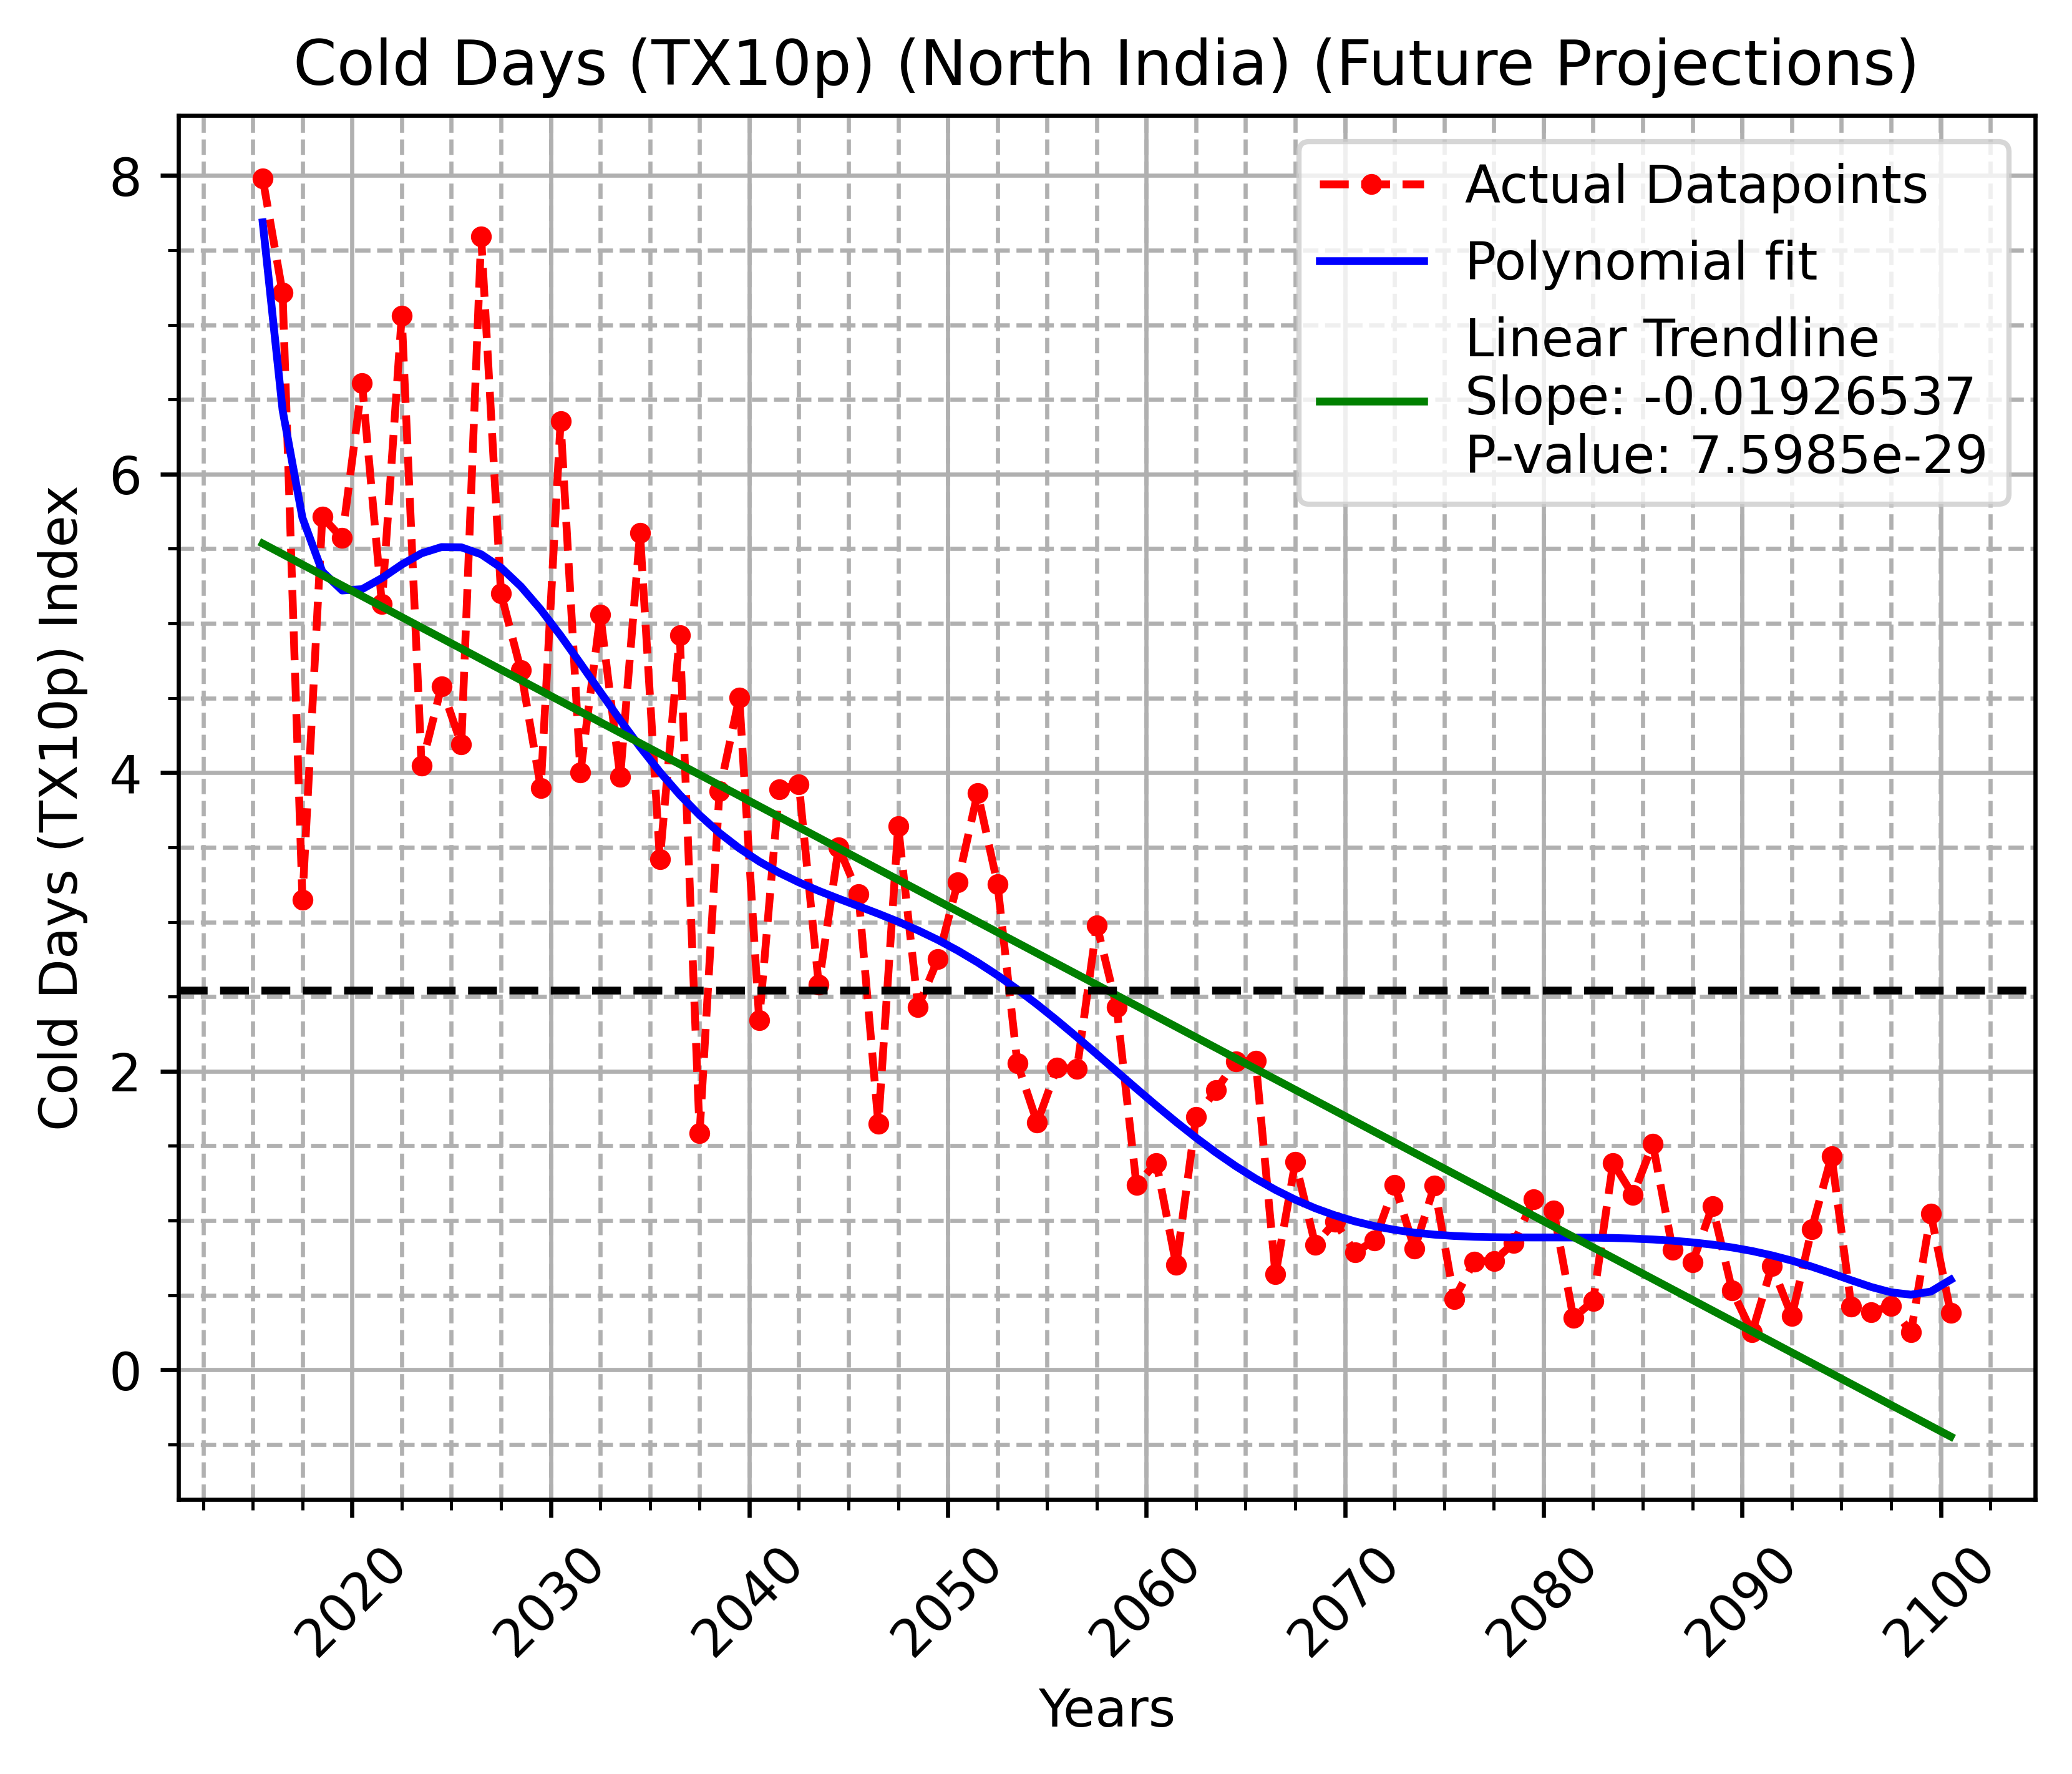
\includegraphics[width=0.95\textwidth]{/home/shiv/Documents/GitHub/EES405/assignment_4/plots/tx10p.north_india_fut.png}
    \caption{\centering Timeseries plot of TX10p index from 1851-2014 (Future epoch) over North India (72E-80E, 29-37N)}
    \label{fig:TX10p_timeseries_north_india_fut}
\end{figure}

From the above plot, we can infer that the frequency of cold days is decreasing over time in the North Indian region. This could be interpreted as a sign of increasing temperatures or more frequent heatwaves in the coming future epoch and thus increasing the frequency of heatwaves. This increasing temperature can be attributed to the increasing anthropogenic emissions of greenhouse gases in the atmosphere. We also observe that the decadal decrease in the percentage of cold days is more pronounced in the future epoch than the historical epoch. This could be attributed to the fact that the anthropogenic emissions of greenhouse gases in the atmosphere are increasing at a faster rate in the future epoch than the historical epoch. This is in agreement with the increase in anthropogenic greenhouse gases in the atmosphere which is causing the global warming and hence the decrease in the frequency of cold days in the future.
% \newpage
\subsection{Central India (75E-85E, 18-29N) timeseries plot of TX10p index}

\begin{figure}[h]
    \centering
    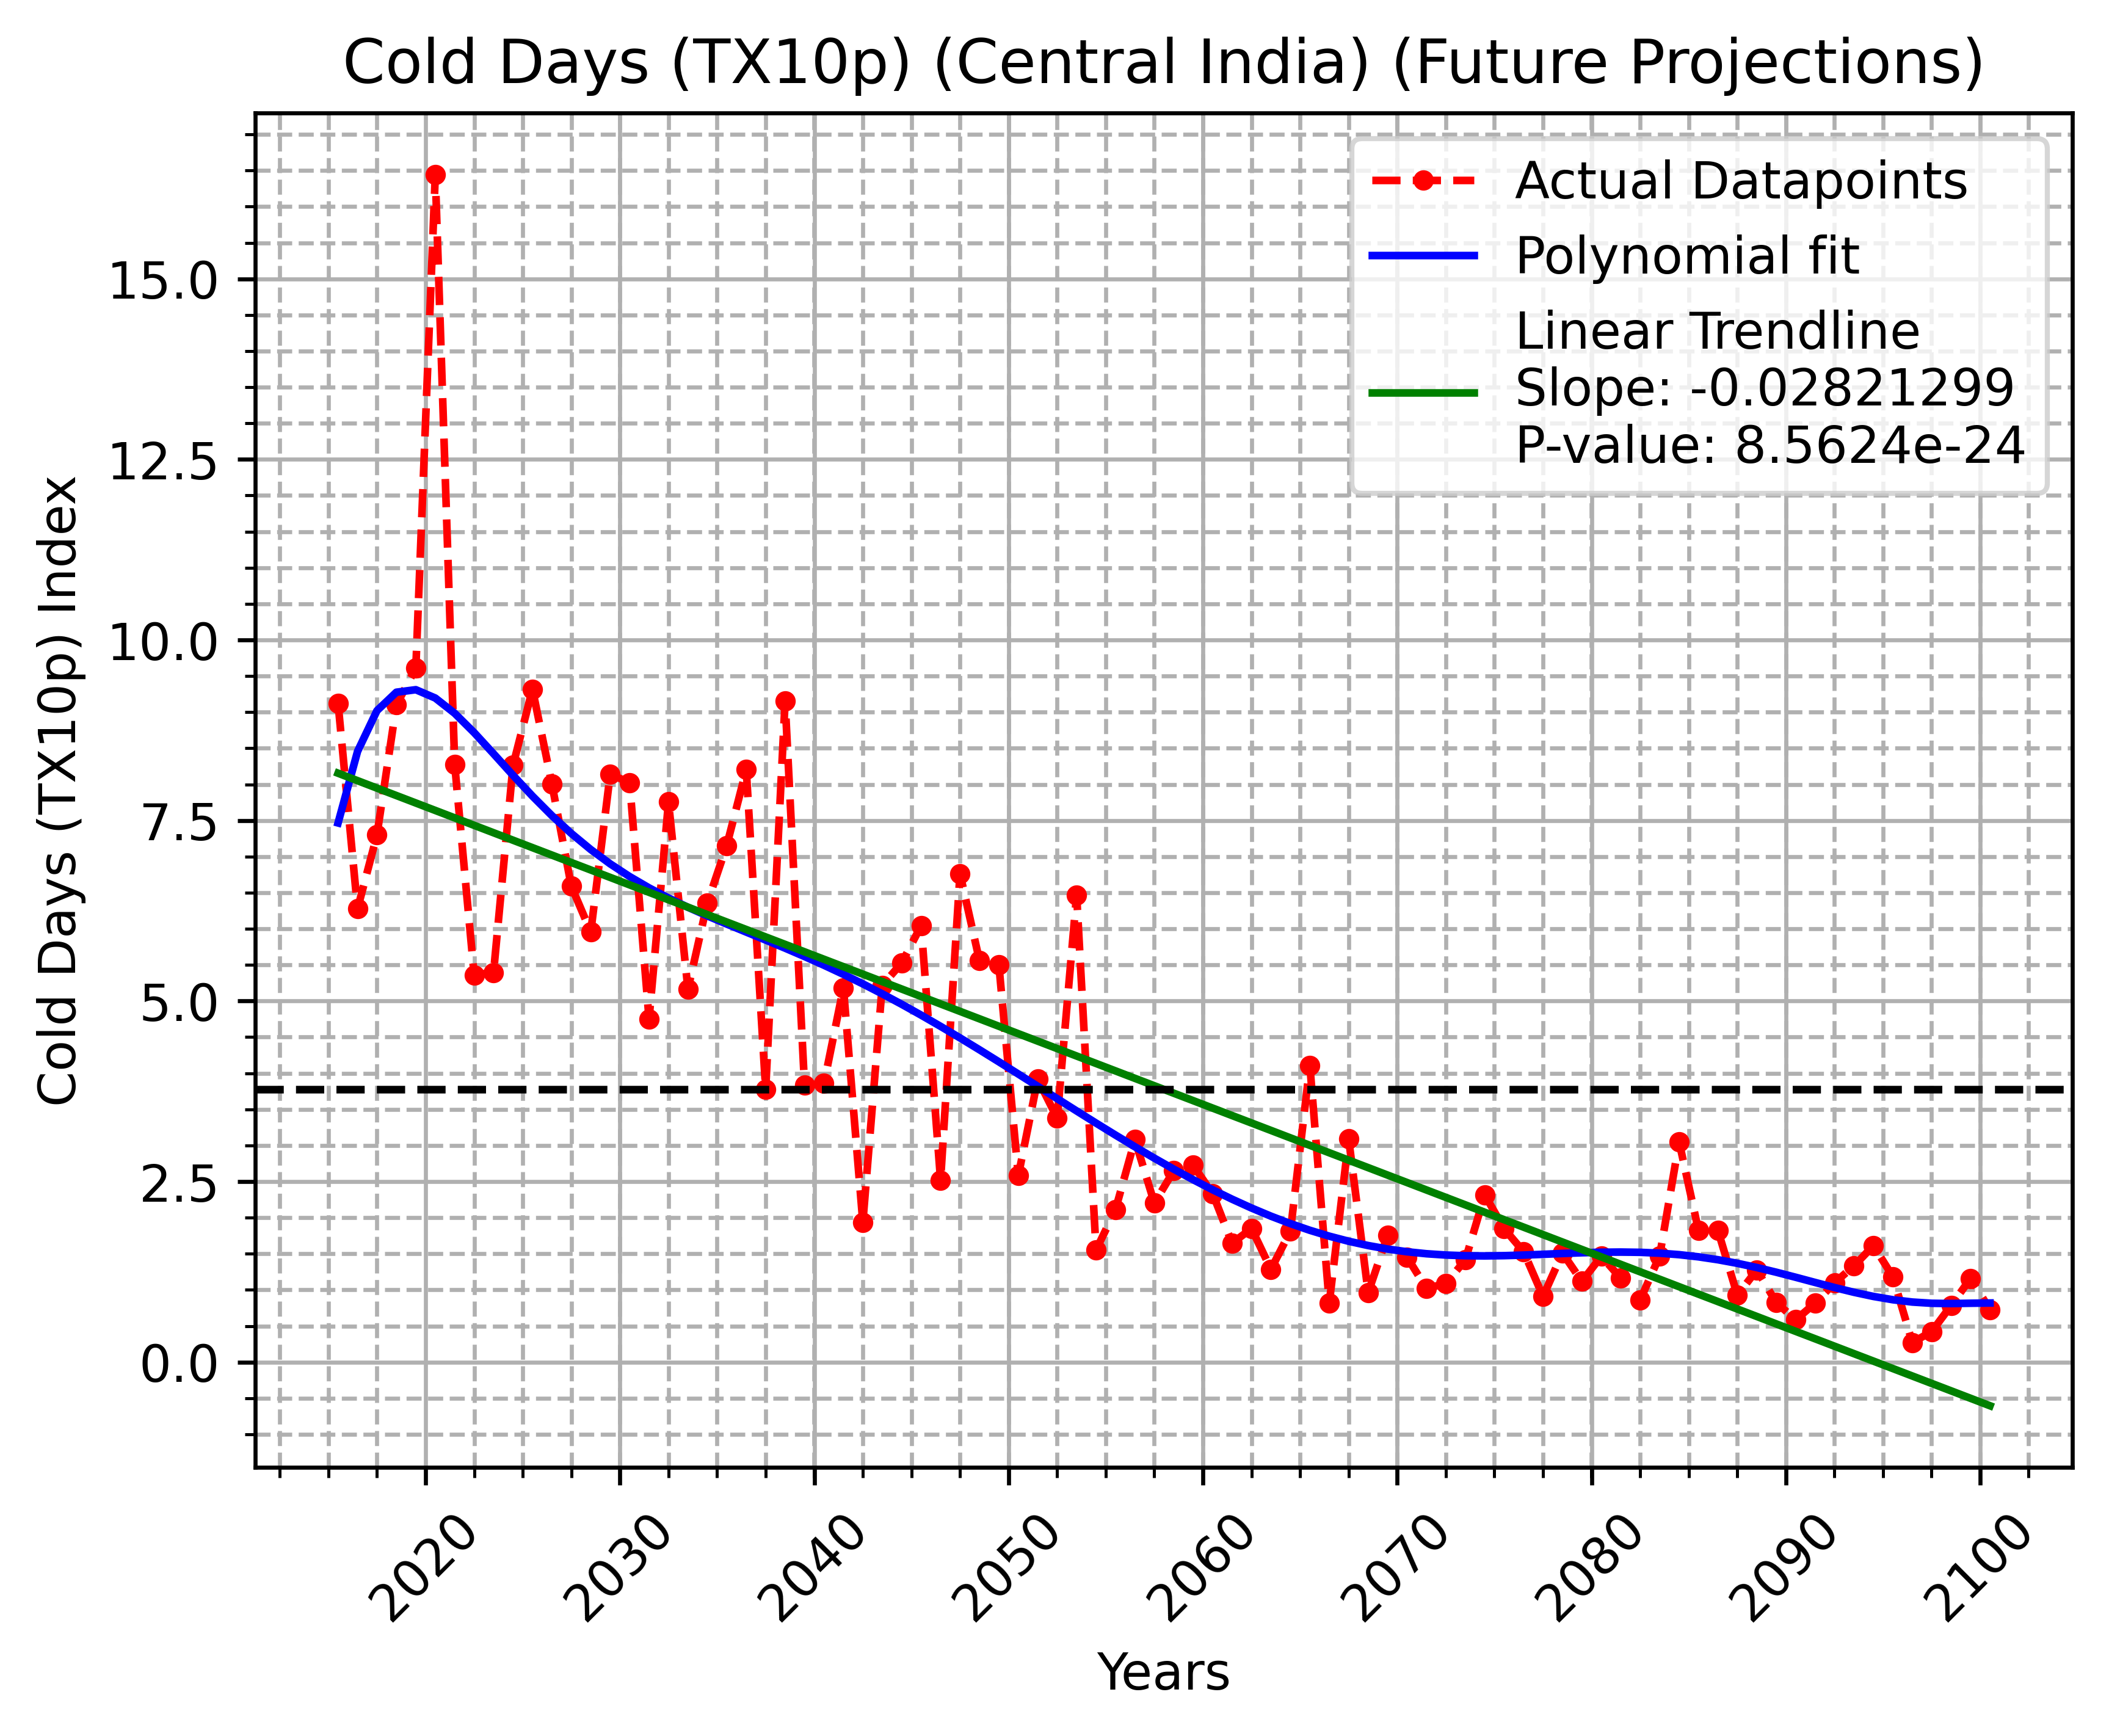
\includegraphics[width=0.95\textwidth]{/home/shiv/Documents/GitHub/EES405/assignment_4/plots/tx10p.central_india_fut.png}
    \caption{\centering Timeseries plot of TX10p index from 1851-2014 (Future epoch) over Central India (72E-80E, 29-37N)}
    \label{fig:TX10p_timeseries_central_india_fut}
\end{figure}

We observe a similar trend in the central Indian region as well. The frequency of cold days is decreasing over time in the central Indian region. This could be interpreted as a sign of increasing temperatures or more frequent heatwaves. This increasing temperature can be attributed to the increasing anthropogenic emissions of greenhouse gases in the atmosphere. We also observe that the decadal decrease in the percentage of cold days is more pronounced in the central Indian region than in the North Indian region. This could be attributed to the fact that the central Indian region is more densely populated than the North Indian region and hence more susceptible to the effects of climate change caused due to human influence.
\newpage
\subsection{West India (68E - 75E, 18E - 29.2E) timeseries plot of TX10p index}

\begin{figure}[h]
    \centering
    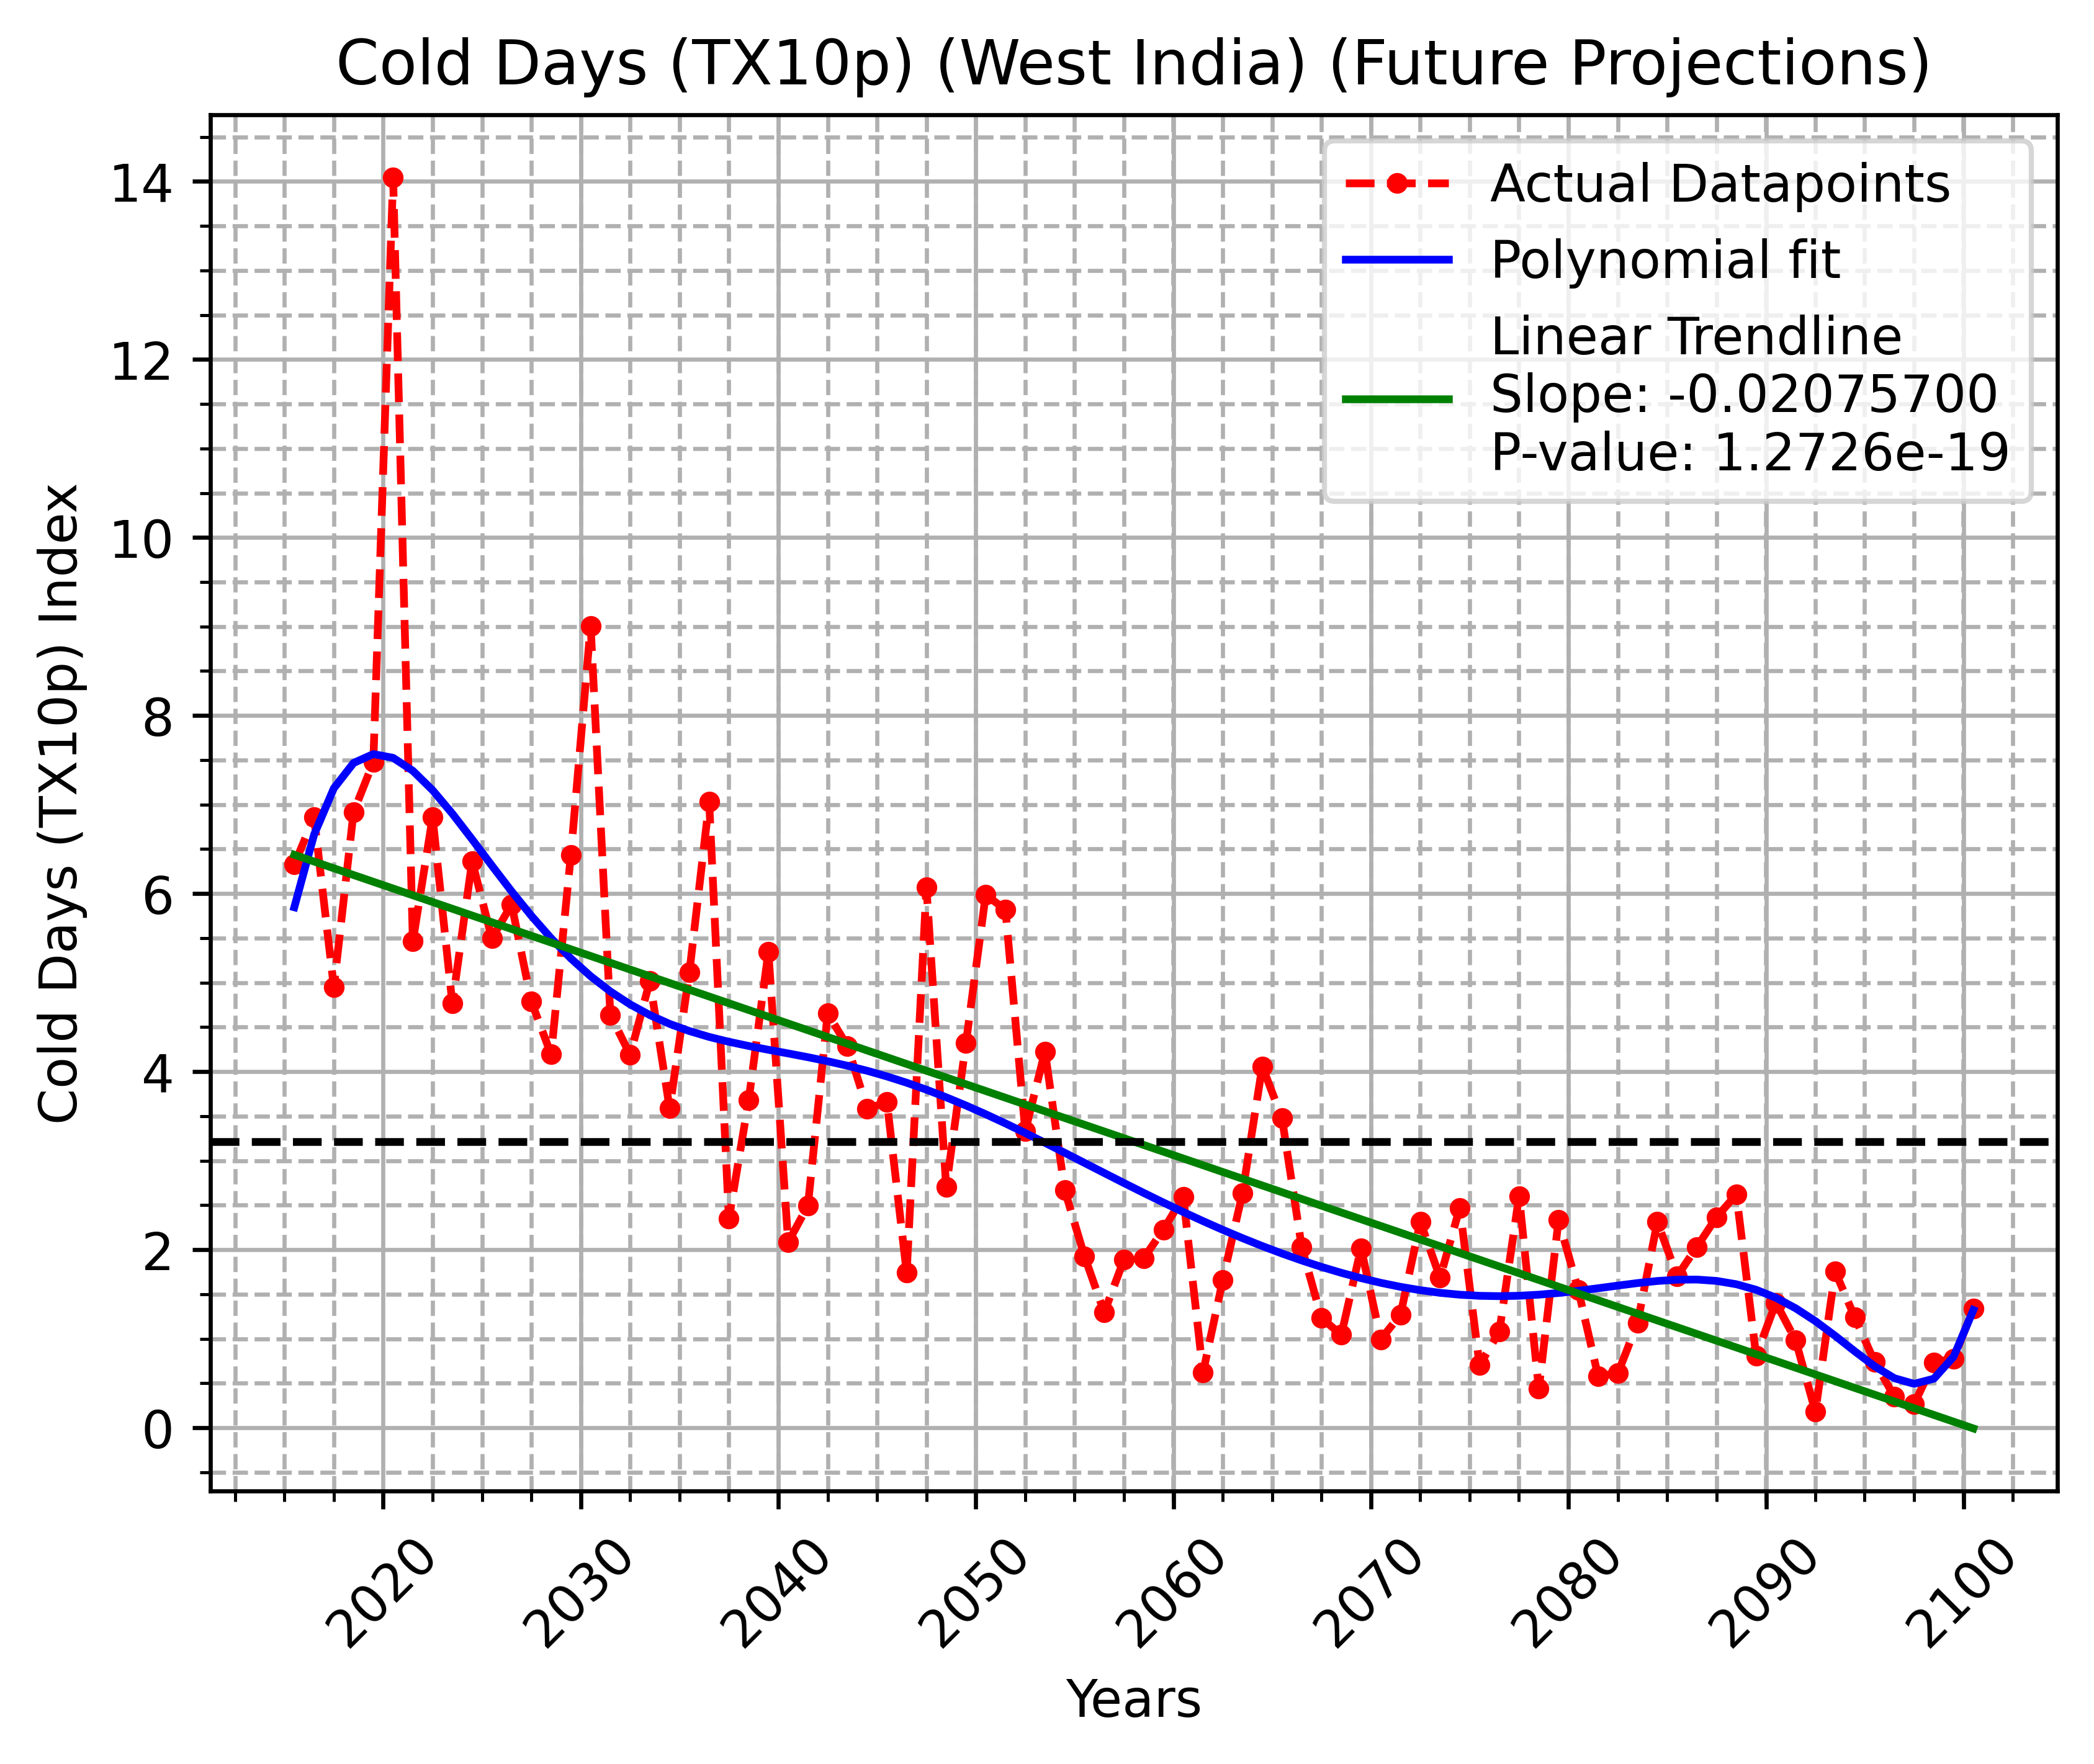
\includegraphics[width=0.95\textwidth]{/home/shiv/Documents/GitHub/EES405/assignment_4/plots/tx10p.west_india_fut.png}
    \caption{\centering Timeseries plot of TX10p index from 1851-2014 (Future epoch) over West India (68E - 75E, 18E - 29.2E)}
    \label{fig:TX10p_timeseries_west_india_fut}
\end{figure}

In the above plot, we see a similar trend of decreasing cold days as expected in western India as well. The frequency of cold days is decreasing over time in the western Indian region. The decadal decrease in the percentage of cold days is almost similar to that of North and central Indian regions. This could be attributed to the fact that the western Indian region contains the most densely populated cities in India and hence more susceptible to the effects of climate change caused due to human influence.
\newpage
\subsection{East India (85E - 97.5E, 19E - 29E) timeseries plot of TX10p index}

\begin{figure}[h]
    \centering
    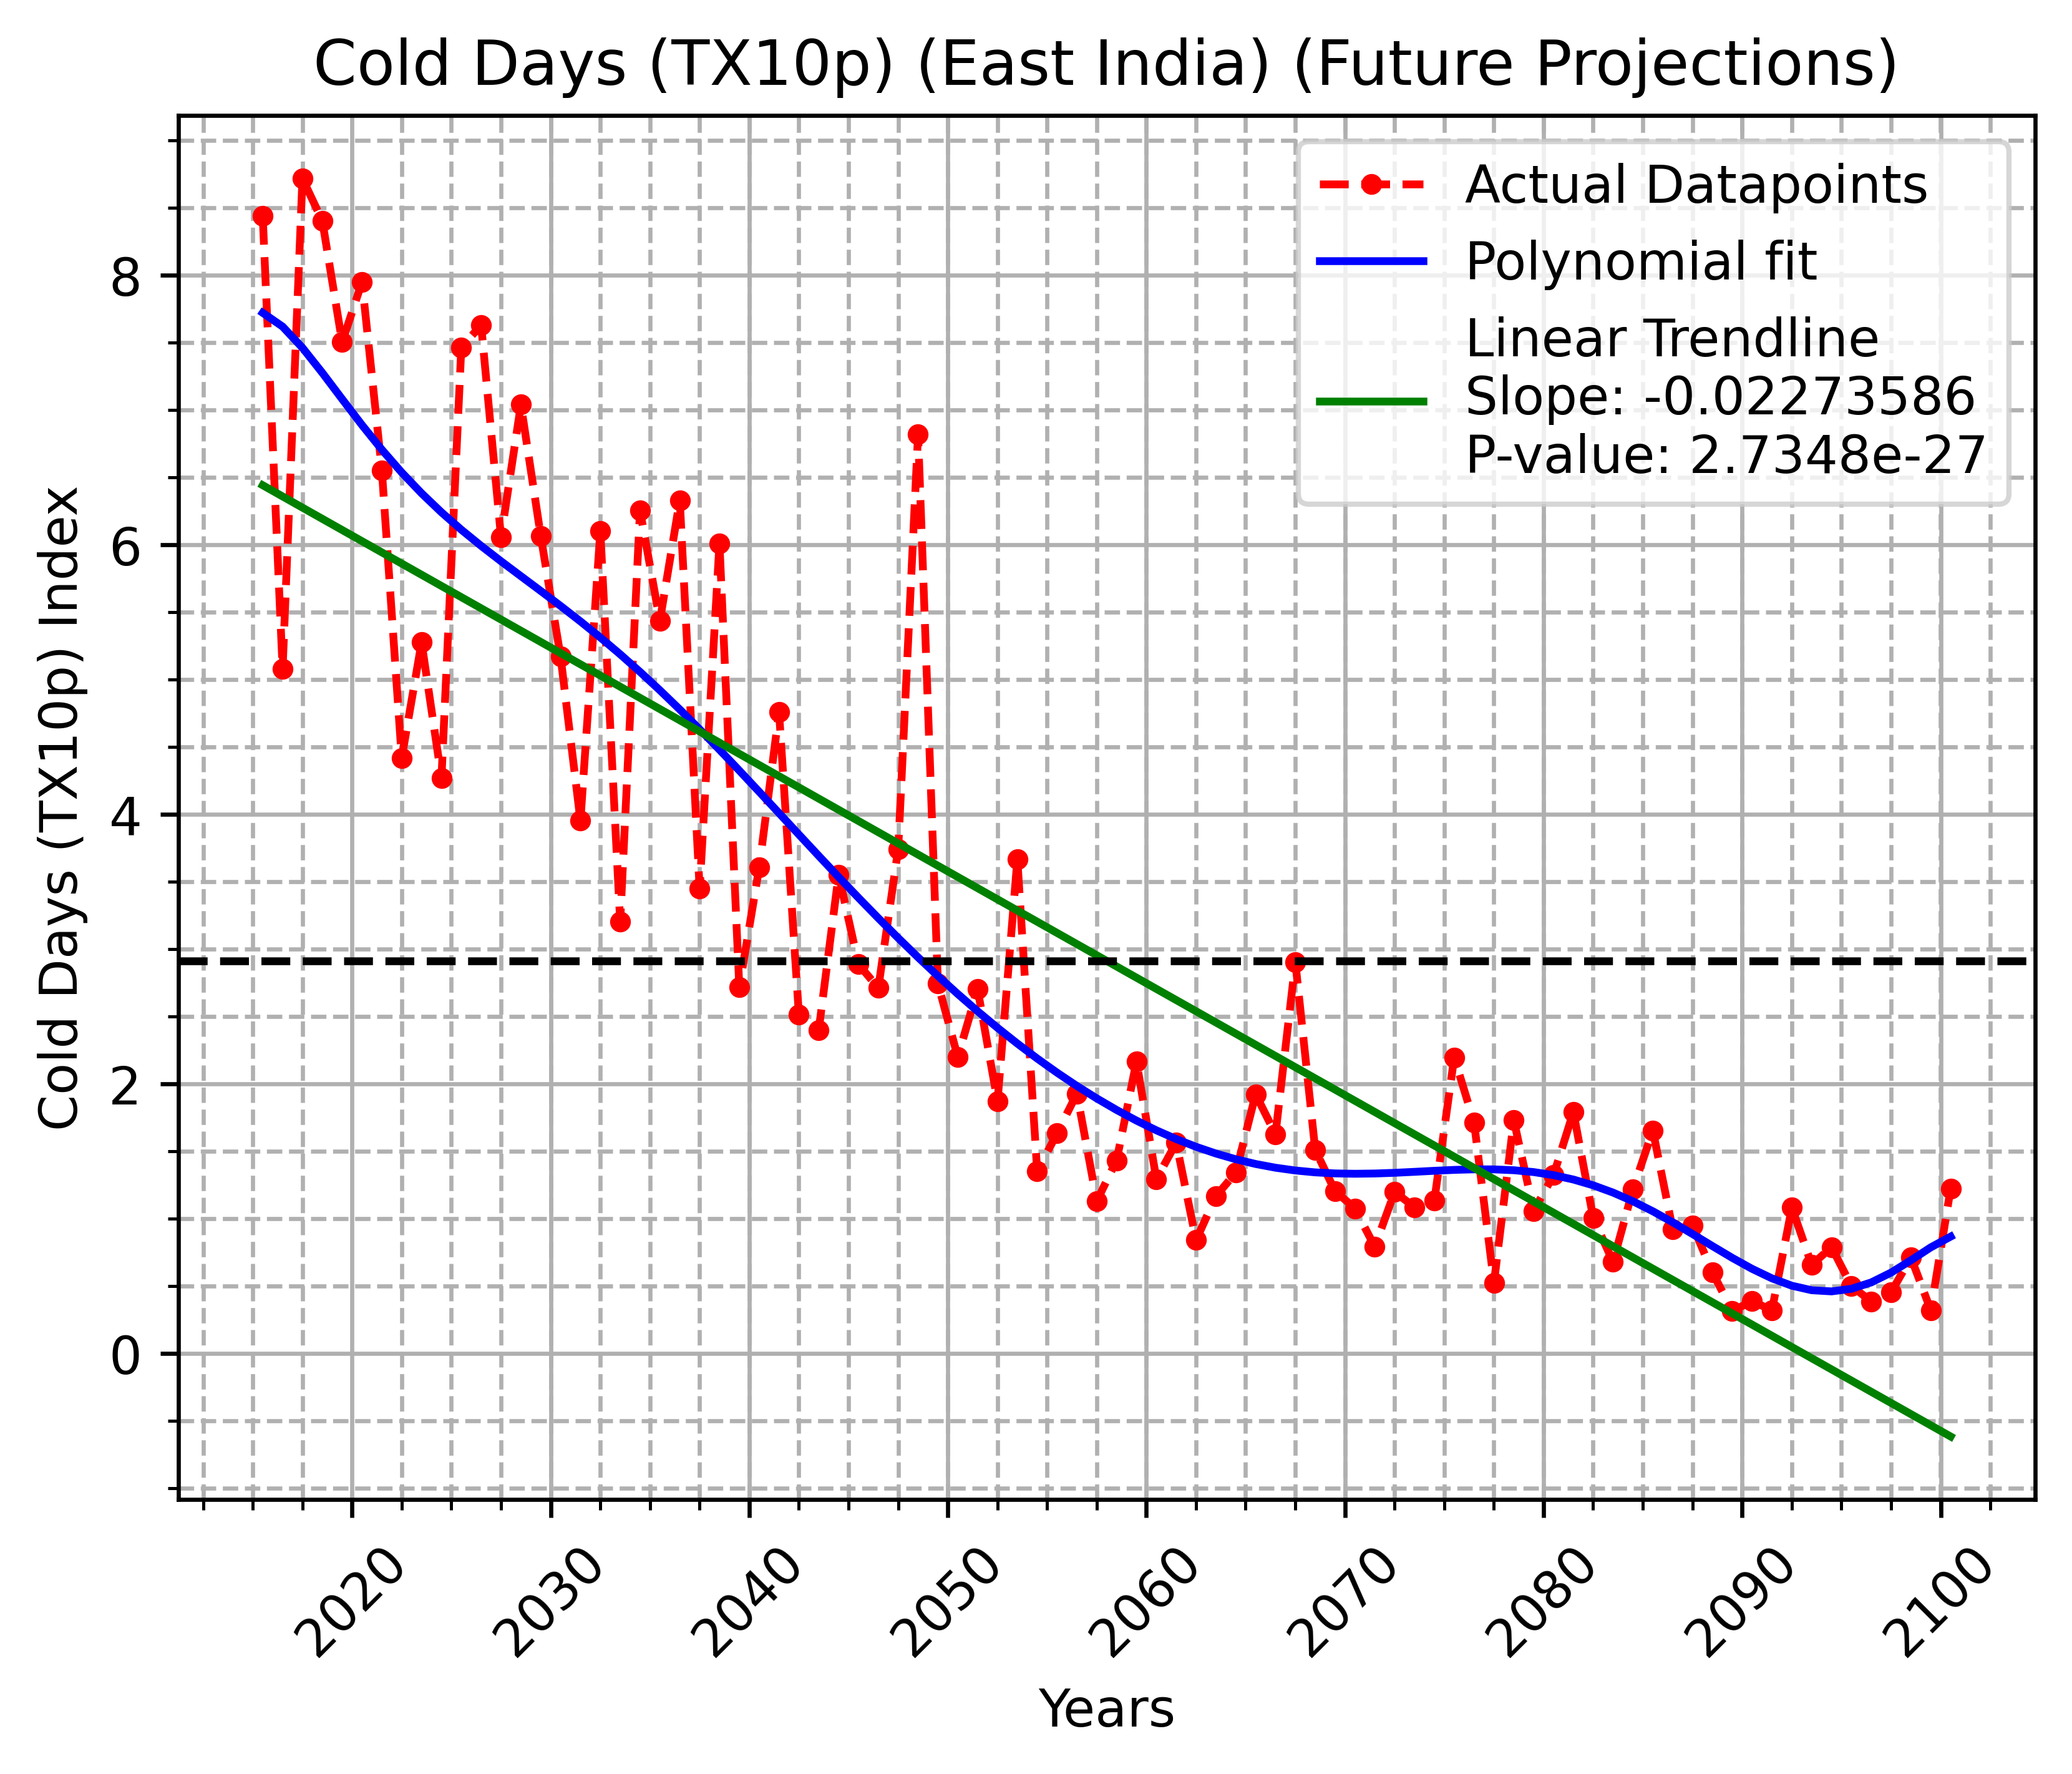
\includegraphics[width=0.95\textwidth]{/home/shiv/Documents/GitHub/EES405/assignment_4/plots/tx10p.east_india_fut.png}
    \caption{\centering Timeseries plot of TX10p index from 1851-2014 (Future epoch) over East India (85E - 97.5E, 19E - 29E)}
    \label{fig:TX10p_timeseries_east_india_fut}
\end{figure}

In the above plot, we see a similar trend of decreasing cold days as expected in eastern India as well. The frequency of cold days is decreasing over time in the eastern Indian region. The decadal decrease in the percentage of cold days is second most after central Indian region showing that effect of climate change is more pronounced in the eastern Indian region owing to various anthropogenic factors.

\newpage

\subsection{South India (73E - 83E, 8E - 18E) timeseries plot of TX10p index}

\begin{figure}[h]
    \centering
    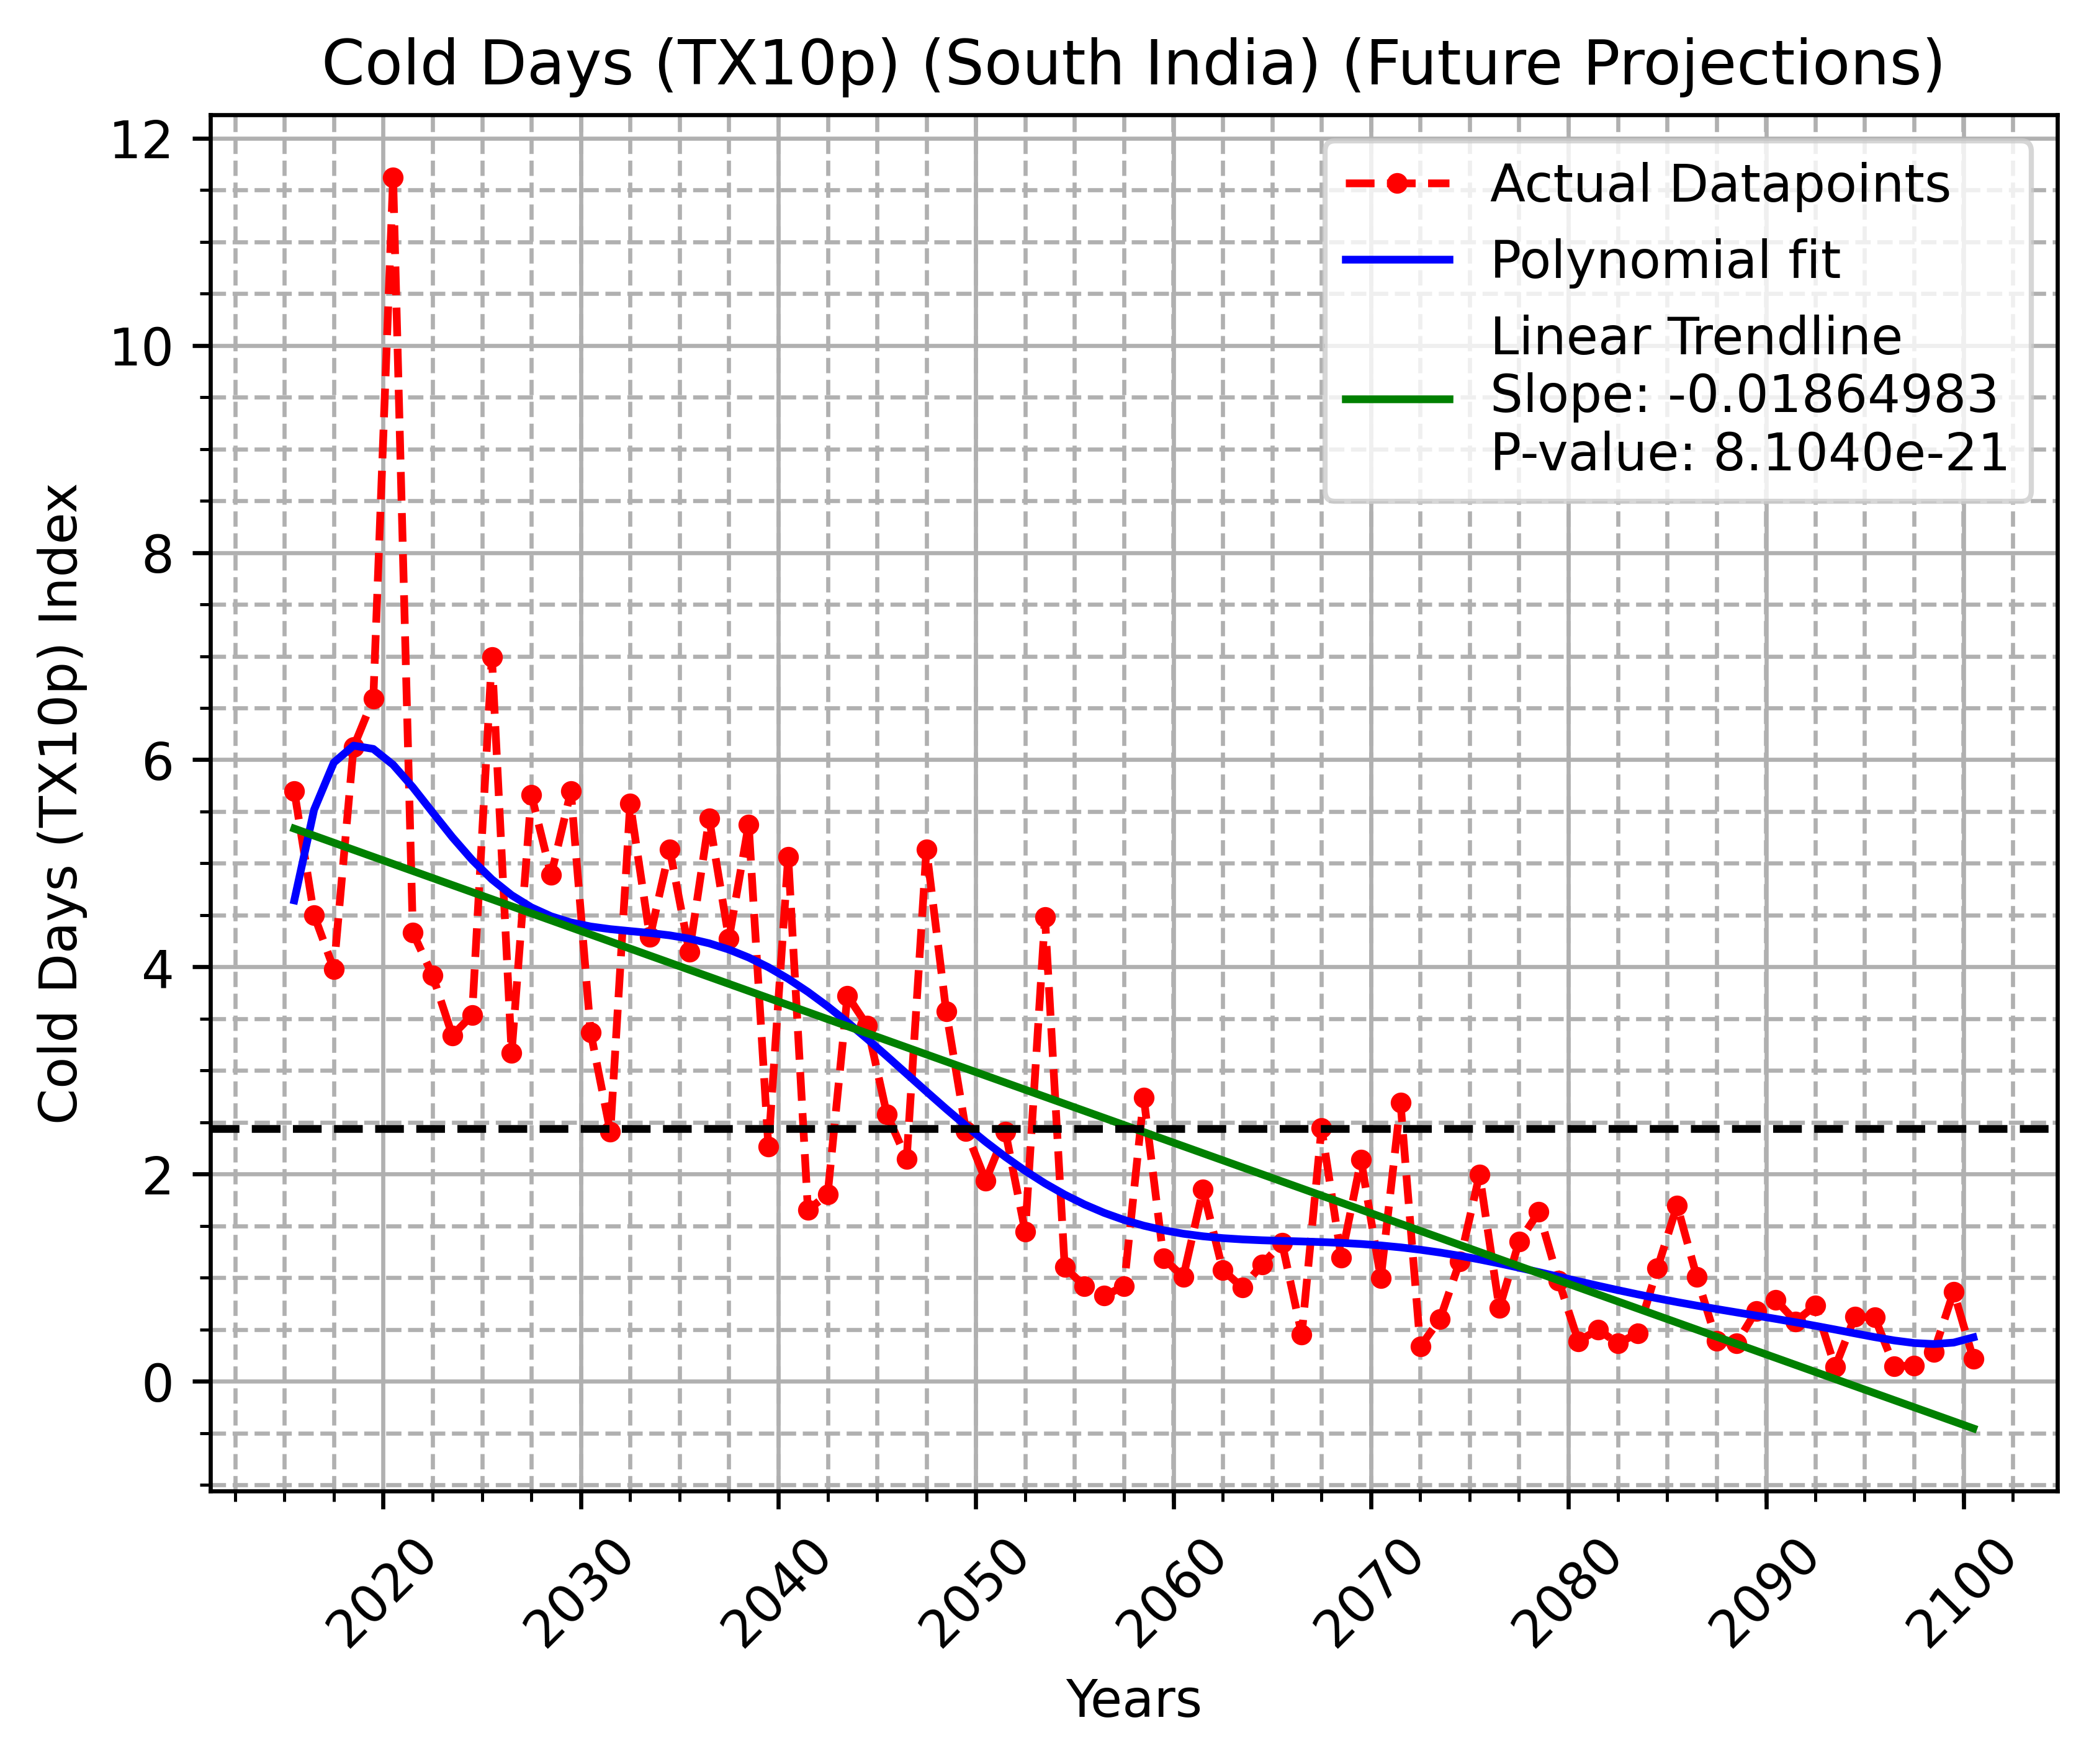
\includegraphics[width=0.95\textwidth]{/home/shiv/Documents/GitHub/EES405/assignment_4/plots/tx10p.south_india_fut.png}
    \caption{\centering Timeseries plot of TX10p index from 1851-2014 (Future epoch) over South India (73E - 83E, 8E - 18E)}
    \label{fig:TX10p_timeseries_south_india_fut}
\end{figure}

In the above plot, we see a similar trend of decreasing cold days as expected in southern India as well. The frequency of cold days is decreasing over time in the southern Indian region. The decadal decrease in the percentage of cold days is least amongst all the Indian regions studied in the present work for future epoch. This could be attributed to the fact that the southern Indian region is already very hot and hence the effect of climate change is less pronounced in this region.

\section{Area averaged (60E-100E, 5-40N) time series of TX10p index from 2015-2100 for different megacities of India}

Indian megacities
\begin{itemize}
    \item Delhi (28N, 77E)
    \item Mumbai (19N, 72E)
    \item Kolkata (22N, 88E)
\end{itemize}
\subsection{Delhi (77E, 28N) timeseries plot of TX10p index}

\begin{figure}[h]
    \centering
    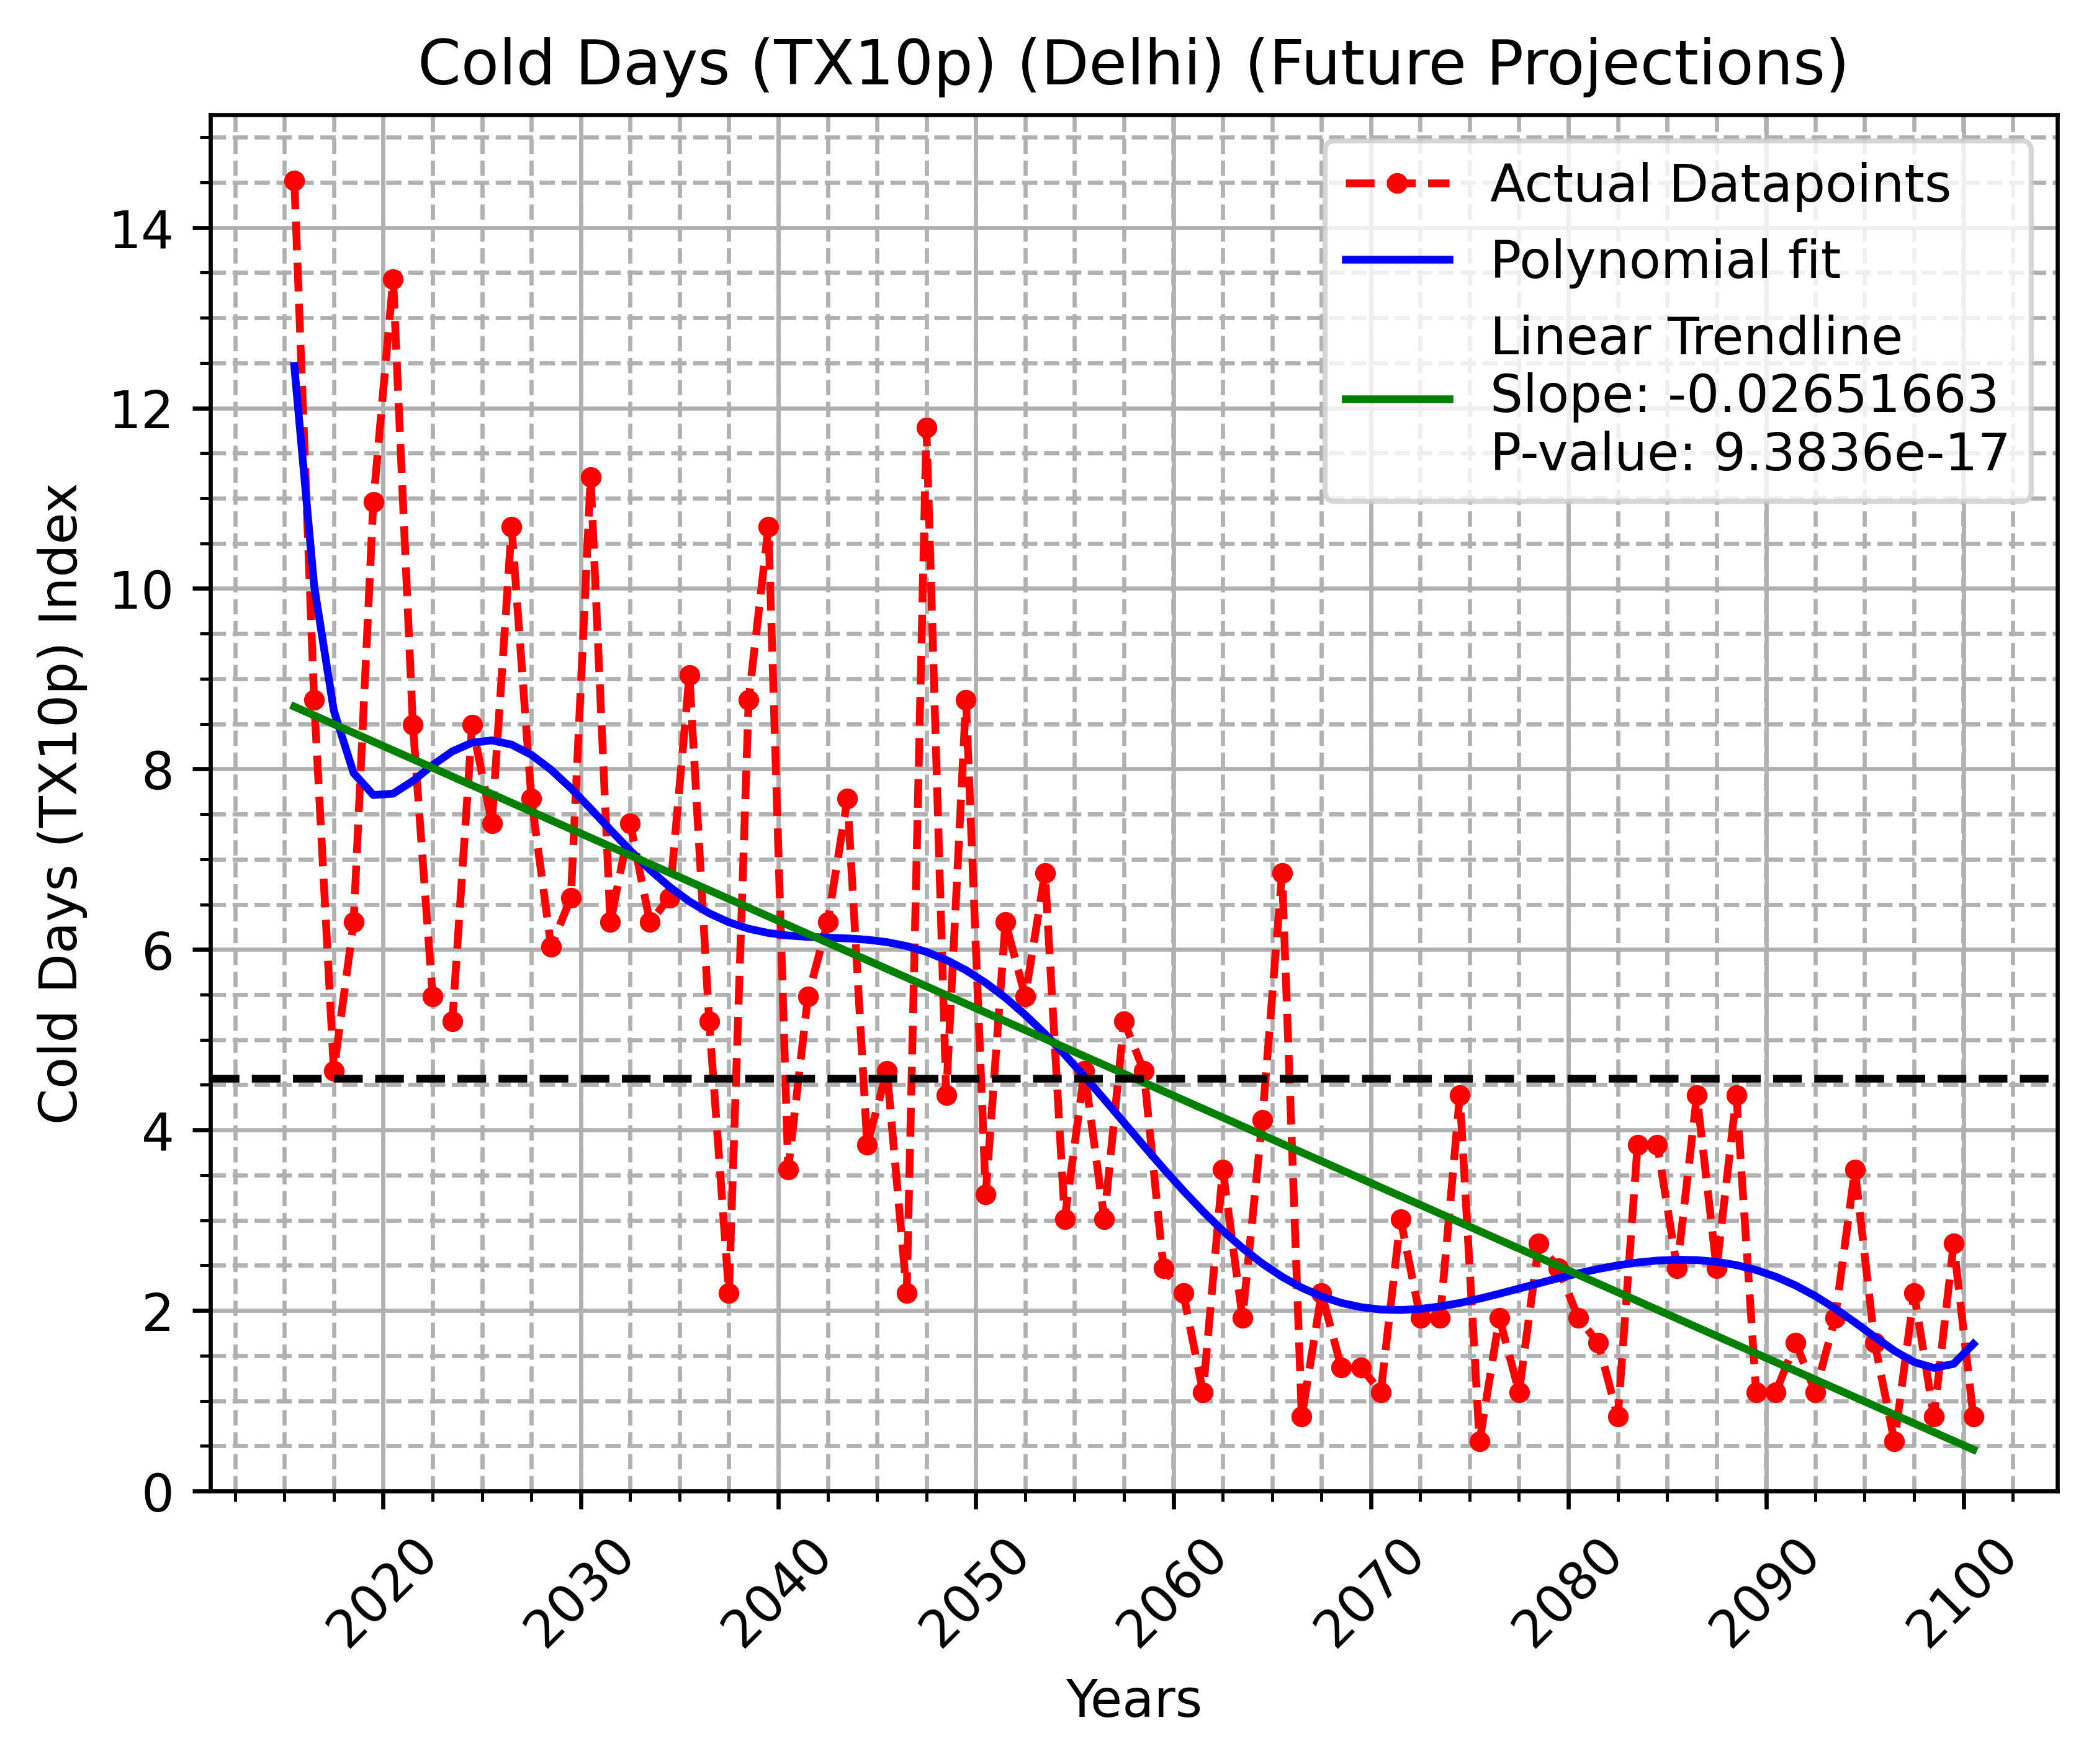
\includegraphics[width=0.95\textwidth]{/home/shiv/Documents/GitHub/EES405/assignment_4/plots/tx10p.delhi_fut.png}
    \caption{\centering Timeseries plot of TX10p index from 2015-2100 (Future epoch) over Delhi (77E, 28N)}
    \label{fig:TX10p_timeseries_delhi_fut}
\end{figure}

In the above plot, we see a similar trend of decreasing cold days as expected in Delhi as well. The frequency of cold days is decreasing over time in the Delhi region. The decadal decrease in the percentage of cold days is similar as compared to other megacities of India.


\newpage

\subsection{Mumbai (72E, 19N) timeseries plot of TX10p index}

\begin{figure}[h]
    \centering
    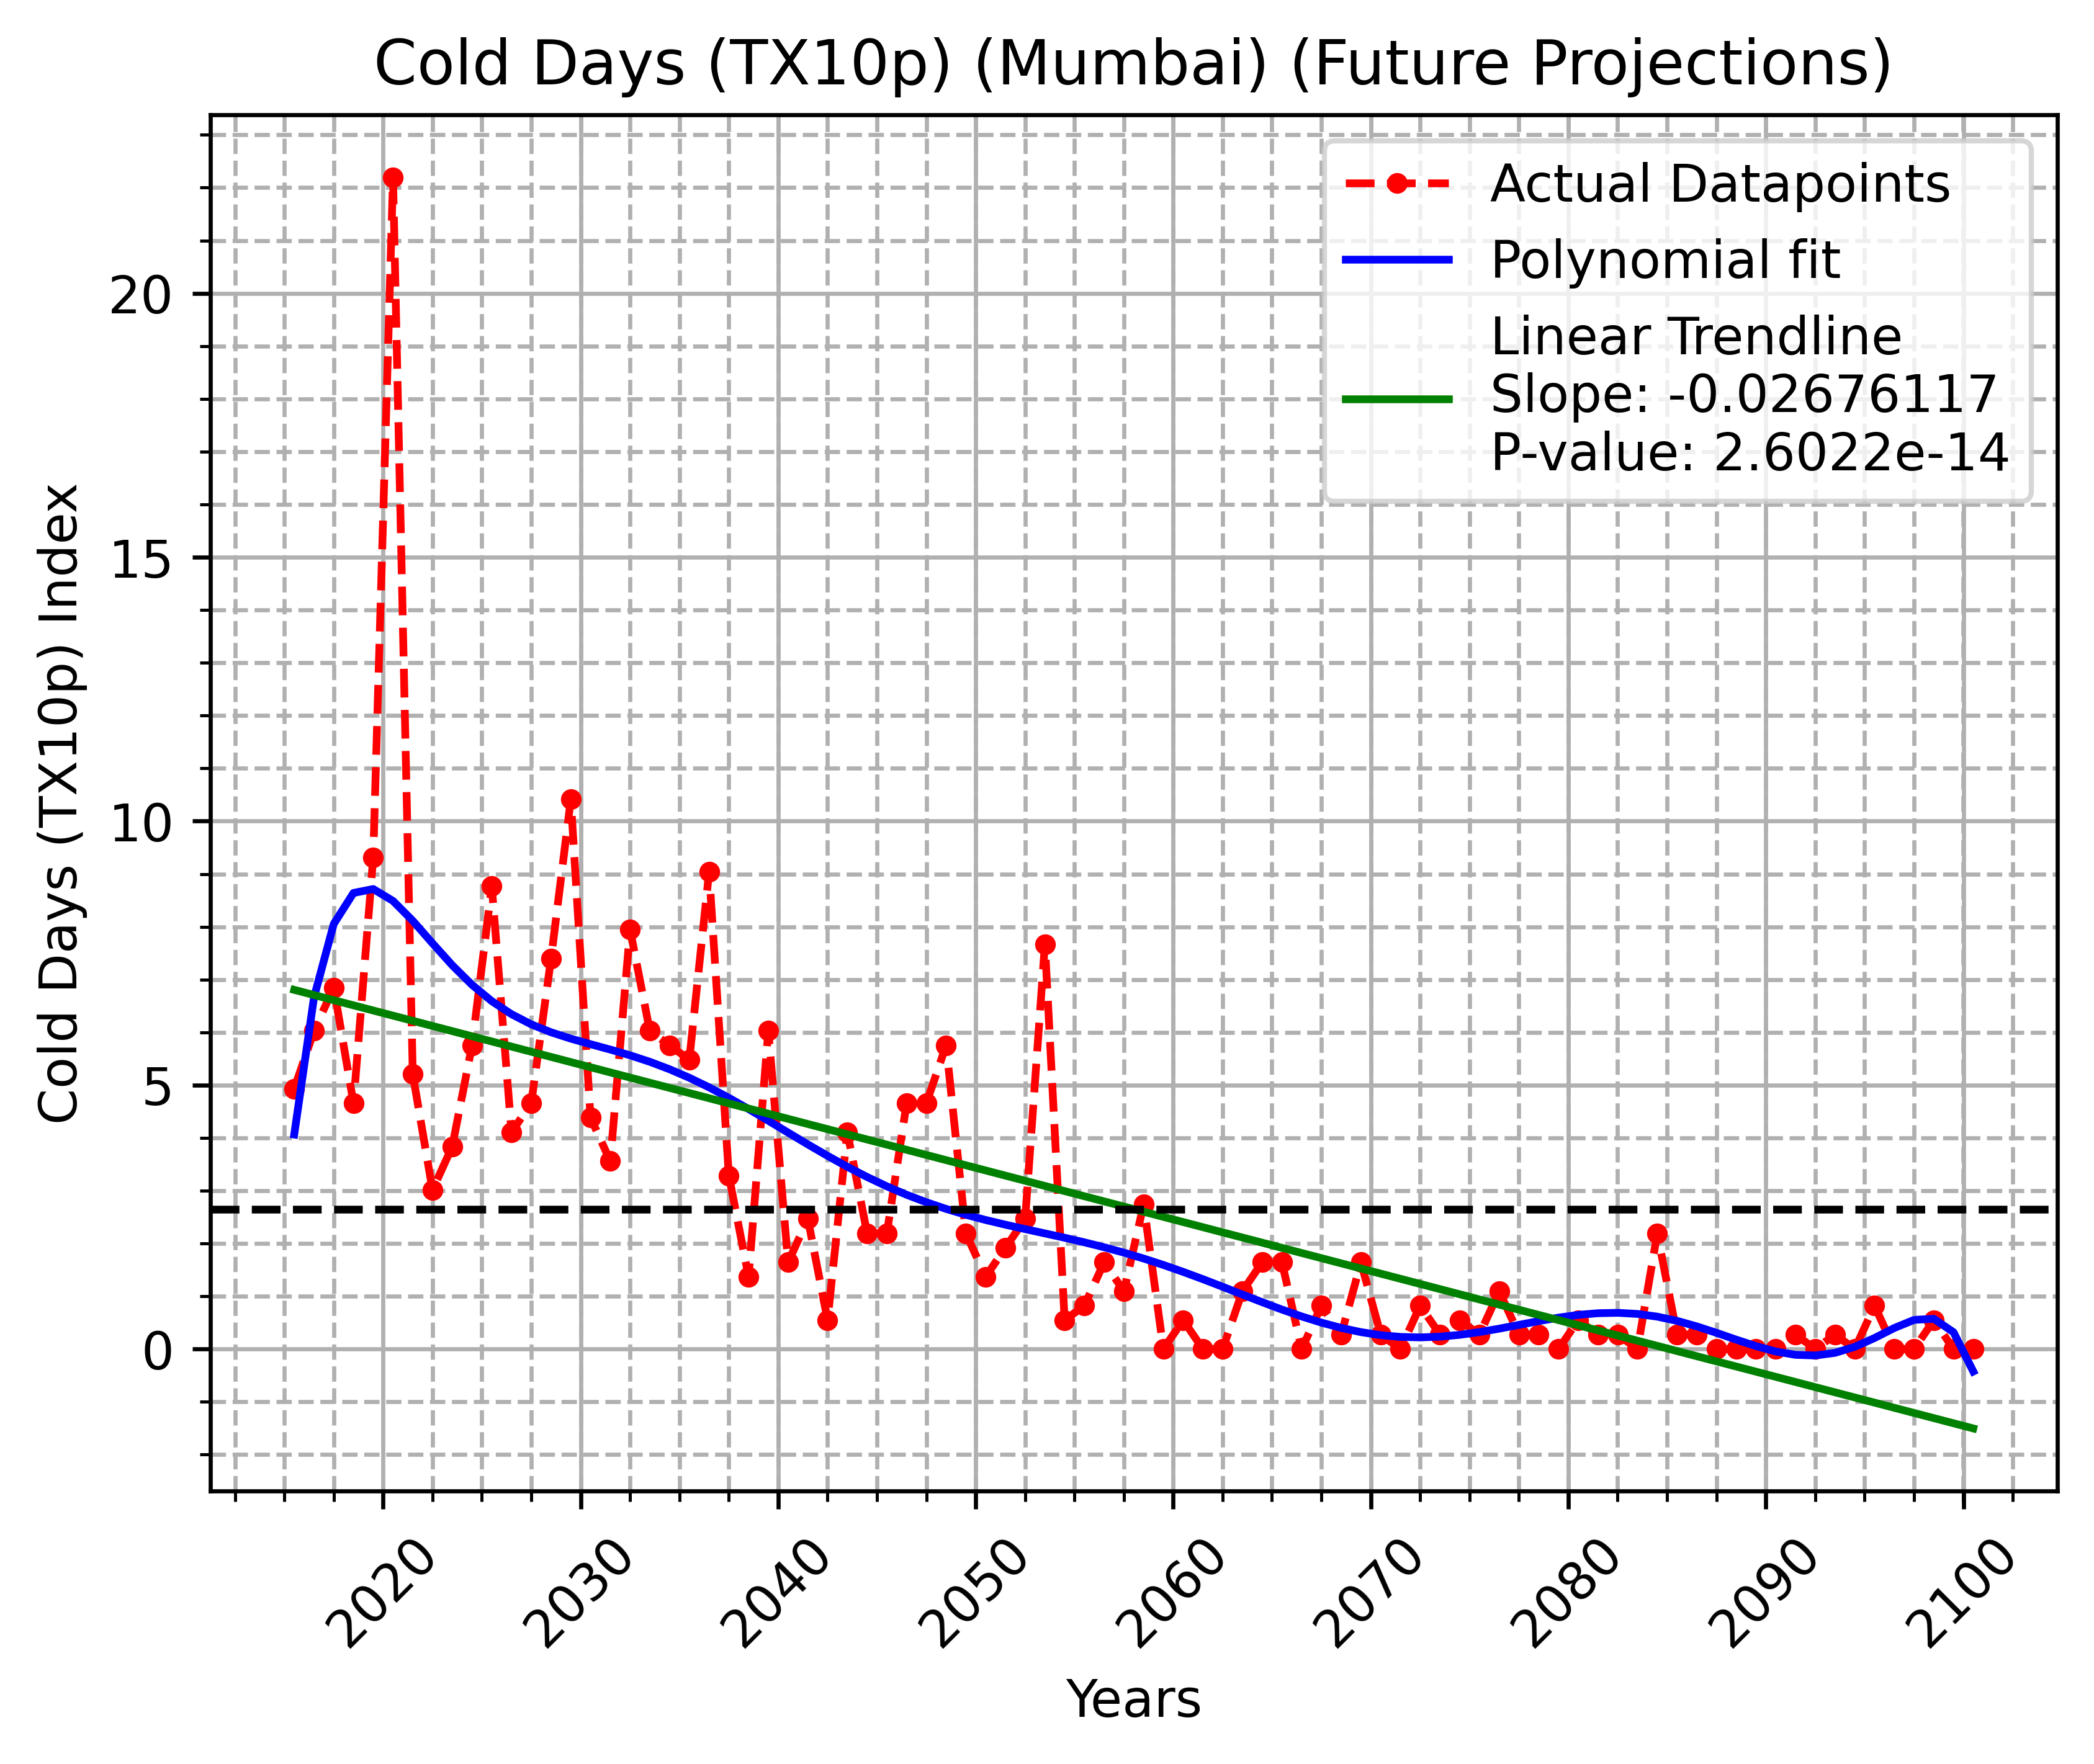
\includegraphics[width=0.95\textwidth]{/home/shiv/Documents/GitHub/EES405/assignment_4/plots/tx10p.mumbai_fut.png}
    \caption{\centering Timeseries plot of TX10p index from 2015-2100 (Future epoch) over Mumbai (72E, 19N)}
    \label{fig:TX10p_timeseries_mumbai_fut}
\end{figure}

In the above plot, we see a similar trend of decreasing cold days as expected in Delhi as well. The frequency of cold days is decreasing over time in the Delhi region. The decadal decrease in the percentage of cold days is least amongst all the Indian regions studied in the present work for future epoch. This could be attributed to the fact that the Mumbai region is a coastal city and temperature is regularised by the land and sea breeze effects and hence the effect of climate change is less pronounced in this region.

\newpage

\subsection{Kolkata (88E, 22N) timeseries plot of TX10p index}

\begin{figure}[h]
    \centering
    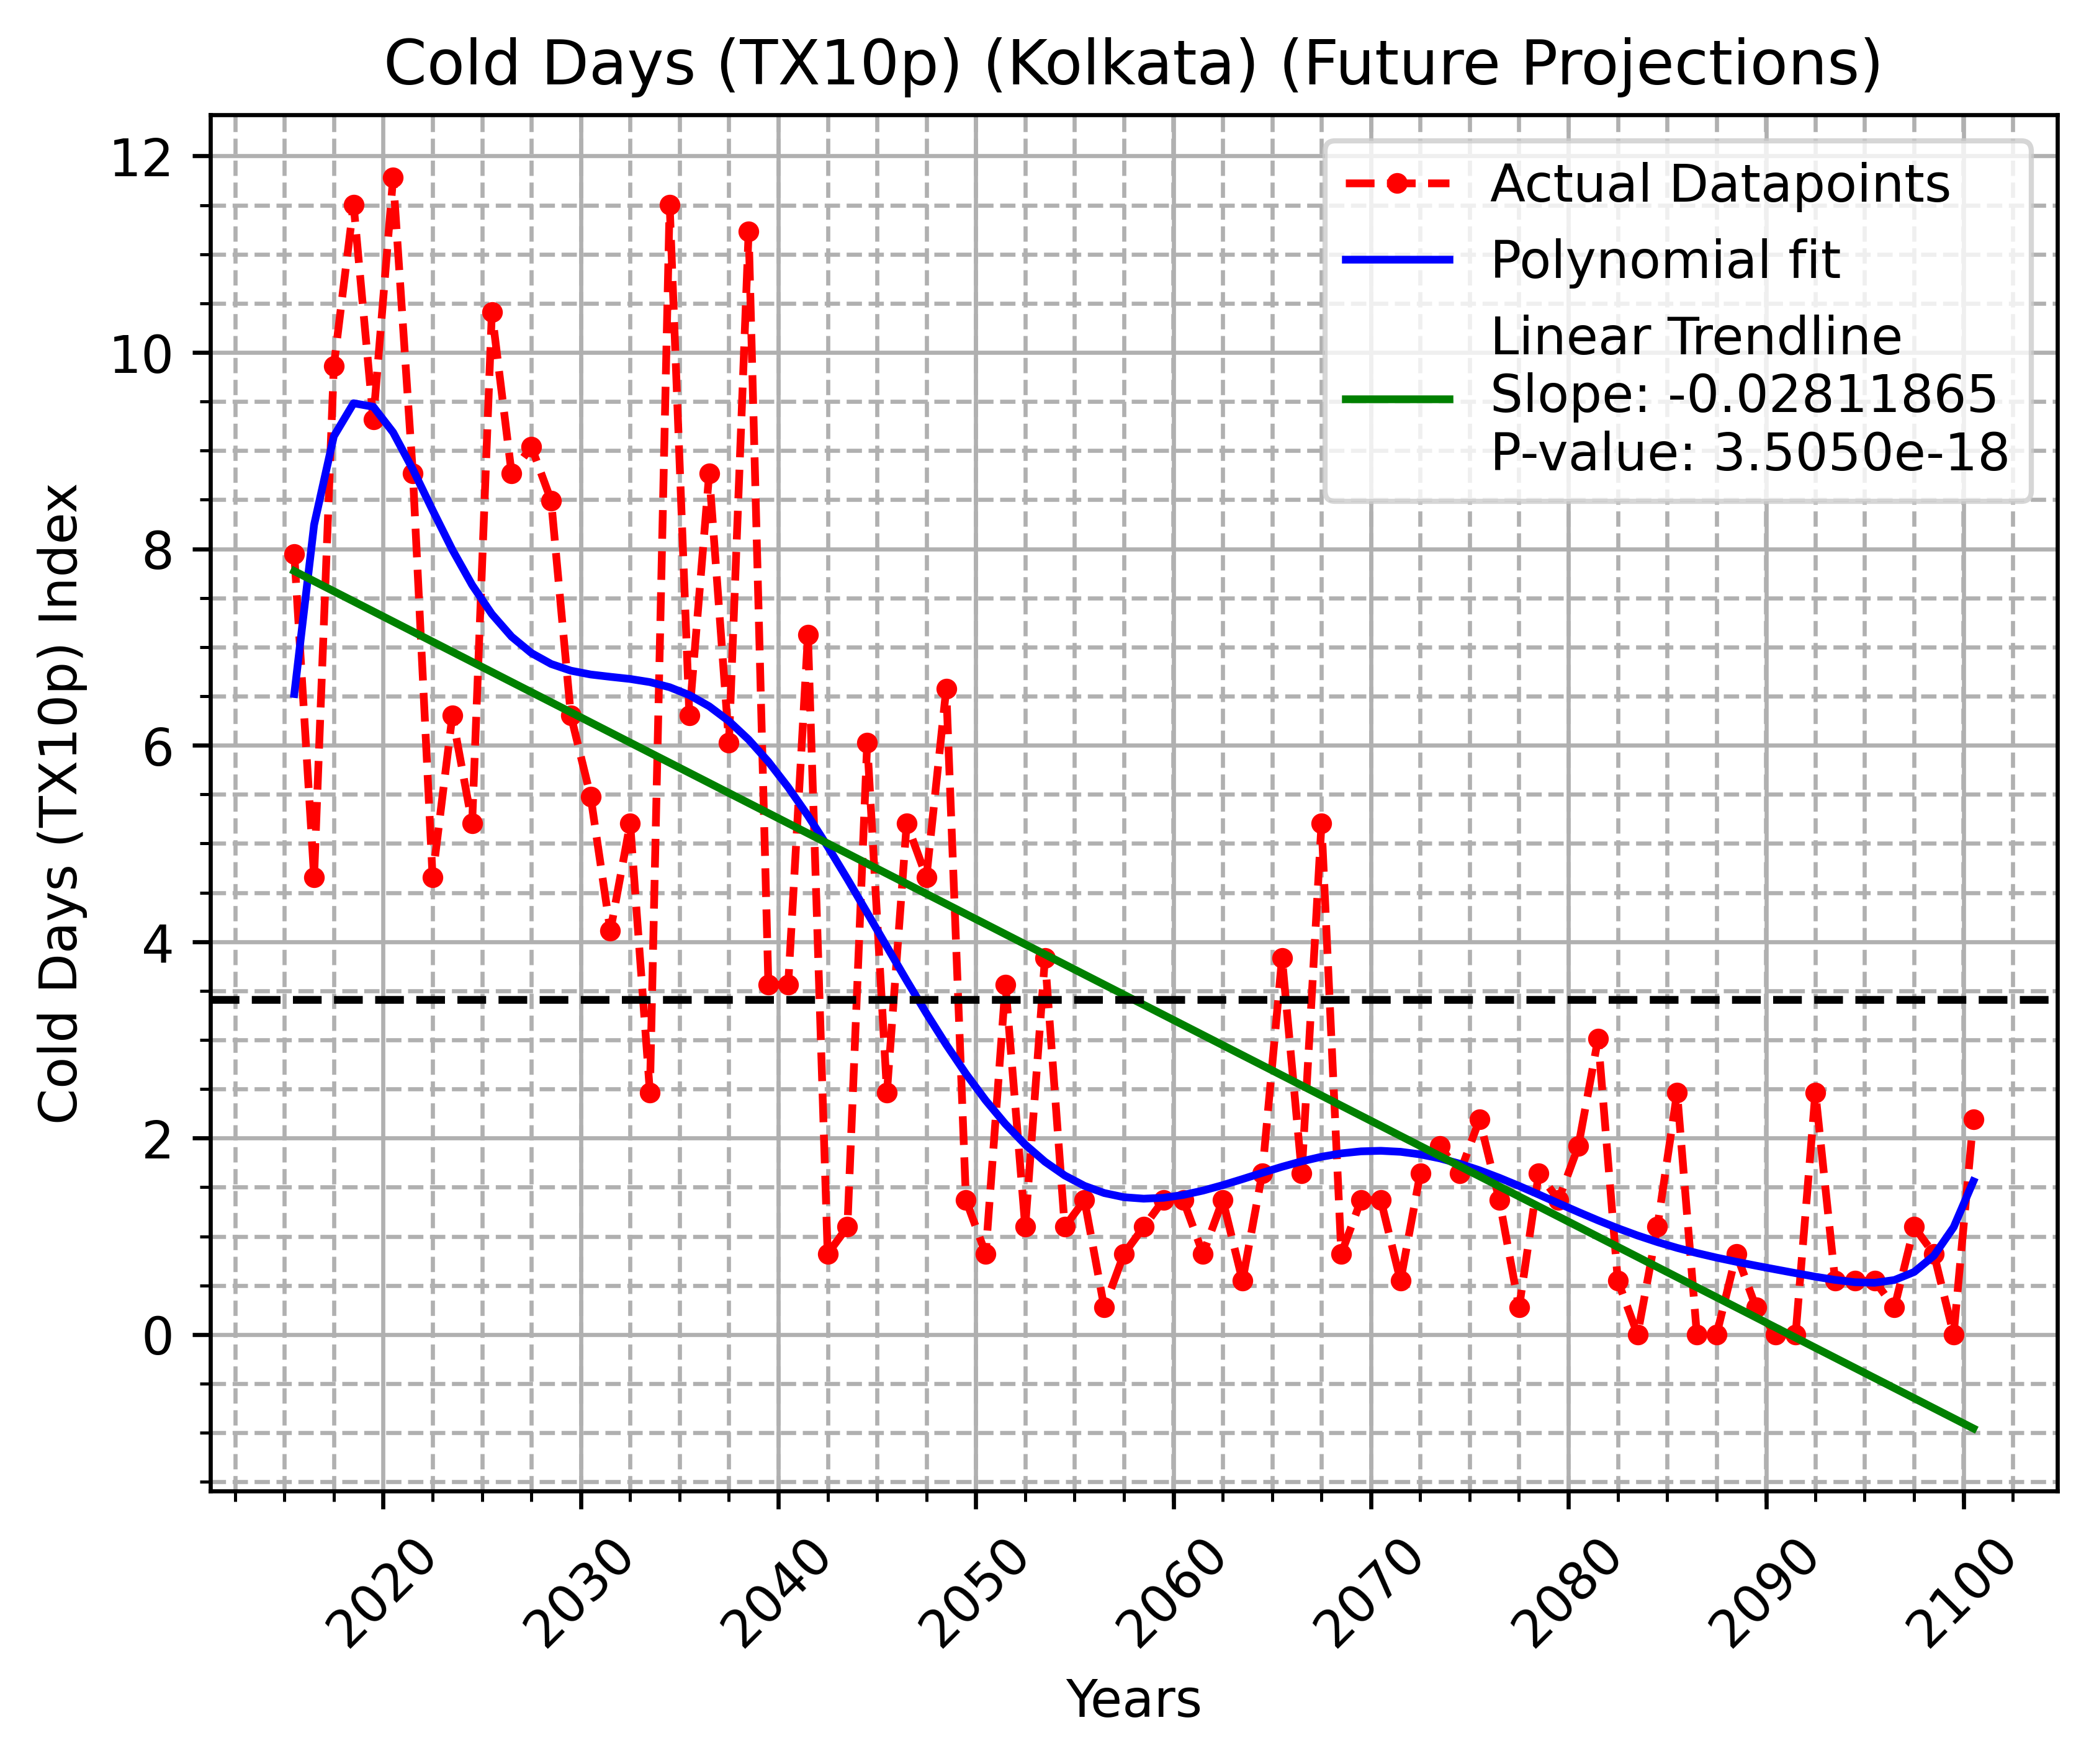
\includegraphics[width=0.95\textwidth]{/home/shiv/Documents/GitHub/EES405/assignment_4/plots/tx10p.kolkata_fut.png}
    \caption{\centering Timeseries plot of TX10p index from 2015-2100 (Future epoch) over Kolkata (88E, 22N)}
    \label{fig:TX10p_timeseries_kolkata_fut}
\end{figure}

In the above plot, we see a similar trend of decreasing cold days as expected in Kolkata as well. The frequency of cold days is decreasing over time in the Kolkata region. The decadal decrease in the percentage of cold days is least amongst all the Indian regions studied in the present work for future epoch. This could be attributed to the fact that the Kolkata region is already very hot and hence the effect of climate change is less pronounced in this region.

\chapter{Analysis of TX10p index for the past and future epochs}

\begin{table}[h]
    \centering
    \caption{Slope data for historical and future epochs in five regions}
    \label{tab:slope-data}
    \begin{tabular}{|c|c|c|}
        \hline
        Region  & \textbf{Historical Slope} & \textbf{Future Slope} \\ \hline
        North   & 0.0042                    & 0.0192                \\ \hline
        West    & 0.0139                    & 0.0207                \\ \hline
        East    & 0.0065                    & 0.0227                \\ \hline
        South   & 0.0147                    & 0.0186                \\ \hline
        Central & 0.0052                    & 0.0282                \\ \hline
    \end{tabular}
\end{table}

All the slope values are calculated for $p<0.05$ \\

From the above table, we can clearly see the decreasing trend of cold days in the past and future epochs. The trend becomes more pronounced in the future epoch as compared to the past epoch. This could be attributed to the fact that the effect of climate change is more pronounced in the future epoch as compared to the past epoch. The slope of the trend line is maximum for the central Indian region and least for the northern Indian region. This could be attributed to the fact that the central Indian region is already very hot and hence the effect of climate change is more pronounced in this region. The northern Indian region is relatively cooler and hence the effect of climate change is less pronounced in this region.

The spatial trend plot for past and future epoch corroborate the same story of decreasing cold days in the past as well as future epochs. The spatial trend analysis is based on \textbf{\textit{Linear Regression model}} and \textbf{\textit{Mann Kendall test}} described in [1]. \\

From the above plots of timeseries and trend we can conclude that as the global temperature increases, it is expected that the number of cold days would decrease, while the number of hot days would increase.

However, it is important to note that this interpretation should be made with caution as the relationship between global warming and cold days is complex and can be influenced by various factors. For instance, changes in regional climate patterns and extreme weather events can also affect the number of cold days. Therefore, it is essential to consider a broader range of factors and analyze long-term trends to accurately assess the impact of global warming on the number of cold days.

\textit{In summary, the decreasing trend of cold days over historical and future epochs, with the most significant decrease in the future epoch, could be indicative of the impact of global warming. However, further analysis is necessary to fully understand the relationship between global warming and the number of cold days.}













\newpage
\appendix


\chapter{Sample Codes}\label{app:appendix1}

%%%
% This code snippet takes care of the required  
% Equation/Figure numbering scheme.
\renewcommand\thefigure{\thechapter.\arabic{figure}}
\renewcommand{\theequation}{\thechapter.\arabic{equation}}
\setcounter{equation}{0}
\setcounter{figure}{0}
%%%

\section{Re-gridding to India shapefile}


\definecolor{dkgreen}{rgb}{0,0.6,0}
\definecolor{gray}{rgb}{0.5,0.5,0.5}
\definecolor{mauve}{rgb}{0.58,0,0.82}

\lstset{frame=tb,
    language=Python,
    aboveskip=3mm,
    belowskip=3mm,
    showstringspaces=false,
    columns=flexible,
    basicstyle={\small\ttfamily},
    numbers=none,
    numberstyle=\tiny\color{gray},
    keywordstyle=\color{blue},
    commentstyle=\color{dkgreen},
    stringstyle=\color{mauve},
    breaklines=true,
    breakatwhitespace=true,
    tabsize=3
}


\begin{lstlisting}
import xarray as xr
import numpy as np
import matplotlib.pyplot as plt
import cartopy.crs as ccrs
import cartopy.feature as cfeature
import geopandas as gpd
import rasterio.features
import pyproj
from shapely.geometry import Point

def create_mask_from_shapefile(dataset, shapefile_gdf):
    lon, lat = np.meshgrid(dataset.lon.values, dataset.lat.values)
    
    # Get the MultiPolygon from the GeoDataFrame
    india_shape = shapefile_gdf.geometry.iloc[0]
    
    mask = np.zeros_like(dataset)

    for i, row in enumerate(lat):
        for j, col in enumerate(lon[0]):
            if india_shape.contains(Point(lon[i, j], lat[i, j])):
                mask[i, j] = 1

    return mask

spatial_data = xr.open_dataset('/home/shiv/Documents/GitHub/EES405/assignment_4/datasets/tx10p.india.future.nc')
spatial_data = spatial_data['tx10pETCCDI']
spatial_data = spatial_data.mean(dim=['time'])
spatial_data = spatial_data.squeeze()

lat = spatial_data.lat
lon = spatial_data.lon

india_shapefile_path = '/home/shiv/Documents/GitHub/EES405/assignment_4/India_Boundary_shapefile/India_Boundary.shp'
india_gdf = gpd.read_file(india_shapefile_path)

mask = create_mask_from_shapefile(spatial_data, india_gdf)
masked_data = spatial_data.where(mask == 1, np.nan)

fig = plt.figure(figsize=(32, 32))
ax = fig.add_subplot(1, 1, 1, projection=ccrs.PlateCarree(central_longitude=0.0, globe=None))

mp = ax.imshow(masked_data, extent=(lon.min(), lon.max(), lat.min(), lat.max()), cmap='jet', origin='lower')
plt.title('Climatology data for tx10p future within India shapefile', fontsize=20)

india_gdf.boundary.plot(ax=ax, linewidth=1, edgecolor='black', transform=ccrs.PlateCarree())

ax.add_feature(cfeature.LAND)
ax.add_feature(cfeature.COASTLINE)
ax.add_feature(cfeature.OCEAN)

cbar = fig.colorbar(mp, shrink=0.5, label='Percentage of days below 10th percentile')
cbar.minorticks_on()

gl = ax.gridlines(draw_labels=True, alpha=0.1)
gl.top_labels = False
gl.right_labels = False
plt.savefig('/home/shiv/Documents/GitHub/EES405/assignment_4/plots/tx10p-future-spatial-shapefile-nan-climatology.png', dpi=1200, bbox_inches='tight')


plt.show()

\end{lstlisting}



\section{Spatial Trend calculation using Linear Regression model}


\begin{lstlisting}
    import netCDF4
import numpy as np
import matplotlib.pyplot as plt
from scipy import stats
from matplotlib.colors import TwoSlopeNorm
import cartopy.crs as ccrs
import cartopy.feature as cfeature
import geopandas as gpd
from shapely.geometry import Point

# Read the NetCDF data and calculate trend and p_values

nc = netCDF4.Dataset('/home/shiv/Documents/GitHub/EES405/assignment_4/datasets/tx10p.india.future.nc')

# extract the dataset for tx10pETCCDI

tx10p = nc.variables['tx10pETCCDI'][:] 

# dimensions of the data
time_dim,lat_dim,lon_dim = tx10p.shape

# arrays to store the trend and p-values
trend = np.zeros((lat_dim,lon_dim))
p_values = np.zeros((lat_dim,lon_dim))

# loop over each grid point 

for lat_idx in range(lat_dim):
    for lon_idx in range(lon_dim):
        
        # calculate data at each grid point
        data = tx10p[:,lat_idx,lon_idx]
        
        # fit a linear regression model to the data
        slope,intercept,r_value,p_value,std_error = stats.linregress(np.arange(time_dim),data)
        
        # append the slope (trend) and p-values in the arrays
        trend[lat_idx,lon_idx] = slope
        p_values[lat_idx,lon_idx] = p_value
        
# visualising the trend using a heatmap or contour 

lat = nc.variables['lat'][:]
lon = nc.variables['lon'][:]


# Normalize the colorbar
max_abs_value = np.max(np.abs(trend))
norm = TwoSlopeNorm(vmin=-0.20, vcenter=0, vmax=0.10)


# Read India boundary shapefile
india_shapefile_path = '/home/shiv/Documents/GitHub/EES405/assignment_4/India_Boundary_shapefile/India_Boundary.shp'
india_gdf = gpd.read_file(india_shapefile_path)

def create_mask_from_shapefile(lon, lat, shapefile_gdf):
    lon_mesh, lat_mesh = np.meshgrid(lon, lat)
    india_shape = shapefile_gdf.geometry.iloc[0]
    mask = np.zeros_like(lat_mesh)

    for i, row in enumerate(lat_mesh):
        for j, col in enumerate(lon_mesh[0]):
            if india_shape.contains(Point(lon_mesh[i, j], lat_mesh[i, j])):
                mask[i, j] = 1

    return mask

# Create mask using the India shapefile
mask = create_mask_from_shapefile(lon, lat, india_gdf)
masked_trend = np.where(mask == 1, trend, np.nan)

# Normalize the colorbar
max_abs_value = np.max(np.abs(masked_trend))
norm = TwoSlopeNorm(vmin=-0.20, vcenter=0, vmax=0.10)

fig = plt.figure(figsize=(32, 32))
ax = fig.add_subplot(1, 1, 1, projection=ccrs.PlateCarree(central_longitude=0.0, globe=None))

mp = ax.imshow(masked_trend, extent=(lon.min(), lon.max(), lat.min(), lat.max()), cmap='coolwarm', origin='lower', norm=norm)
plt.title('Spatial trend data for tx10p future within India shapefile', fontsize=20)

india_gdf.boundary.plot(ax=ax, linewidth=1, edgecolor='black', transform=ccrs.PlateCarree())

ax.add_feature(cfeature.LAND)
ax.add_feature(cfeature.COASTLINE)
ax.add_feature(cfeature.OCEAN)

# Add black dots for significant trends (p < 0.05)
lon_mesh, lat_mesh = np.meshgrid(lon, lat)
significant_trend = np.where((mask == 1) & (p_values < 0.05))
ax.scatter(lon_mesh[significant_trend], lat_mesh[significant_trend], color='black', s=10, transform=ccrs.PlateCarree())


cbar = fig.colorbar(mp, shrink=0.3, label='Trend Slope')
cbar.minorticks_on()

gl = ax.gridlines(draw_labels=True, alpha=0.1)
gl.top_labels = False
gl.right_labels = False

plt.savefig('/home/shiv/Documents/GitHub/EES405/assignment_4/plots/spatial-trend-future-india-shapefile.png', dpi=600, bbox_inches='tight')
plt.show()

\end{lstlisting}



\section{Spatial Trend calculation using Mann Kendall Test}

\begin{lstlisting}
## trying to do mann-kendall test for the trends 
import netCDF4
import numpy as np
import matplotlib.pyplot as plt
import cartopy.crs as ccrs
import cartopy.feature as cfeature
from scipy import stats


from matplotlib.colors import TwoSlopeNorm


nc = netCDF4.Dataset('/home/shiv/Documents/GitHub/EES405/assignment_4/datasets/tx10p.india.future.nc')

# extract the dataset for tx10pETCCDI

tx10p = nc.variables['tx10pETCCDI'][:] 

# dimensions of the data
time_dim,lat_dim,lon_dim = tx10p.shape

# arrays to store the trend and p-values
trend = np.zeros((lat_dim,lon_dim))
p_values = np.zeros((lat_dim,lon_dim))

# loop over each grid point 

import pymannkendall as mk

# Replace the following section of your code
for lat_idx in range(lat_dim):
    for lon_idx in range(lon_dim):
        
        # calculate data at each grid point
        data = tx10p[:,lat_idx,lon_idx]
        
        # Perform the Mann-Kendall test
        result = mk.original_test(data)
        
        # Append the slope (trend) and p-values in the arrays
        trend[lat_idx,lon_idx] = result.slope
        p_values[lat_idx,lon_idx] = result.p

        
# visualising the trend using a heatmap or contour 

lat = nc.variables['lat'][:]
lon = nc.variables['lon'][:]

significant_trends = p_values < 0.05

# Normalize the colorbar
max_abs_value = np.max(np.abs(trend))
norm = TwoSlopeNorm(vmin=-max_abs_value, vcenter=0, vmax=max_abs_value)


fig = plt.figure(figsize=(32, 32))
ax = fig.add_subplot(1, 1, 1, projection=ccrs.PlateCarree(central_longitude=0.0, globe=None))


mp = ax.imshow(trend, extent=(lon.min(), lon.max(), lat.min(), lat.max()), cmap='coolwarm', origin='lower', norm=norm)


# Plot black dots at significant trend locations
for lat_idx in range(lat_dim):
    for lon_idx in range(lon_dim):
        if significant_trends[lat_idx, lon_idx]:
            ax.plot(lon[lon_idx], lat[lat_idx], 'ko', markersize=2, transform=ccrs.PlateCarree())

plt.title('Spatial trend data for tx10p future', fontsize=20)

states_provinces = cfeature.NaturalEarthFeature(
        category='cultural',
        name='admin_1_states_provinces_lines',
        scale='10m',
        facecolor='none')
ax.add_feature(cfeature.BORDERS,edgecolor='black')
ax.add_feature(states_provinces, edgecolor='black')

ax.add_feature(cfeature.LAND)
ax.add_feature(cfeature.COASTLINE)
ax.add_feature(cfeature.OCEAN, zorder = 100)


cbar = fig.colorbar(mp, shrink=0.3,label='Frequency')
cbar.minorticks_on()

#adding the long lat grids and enabling the tick labels
gl = ax.gridlines(draw_labels=True,alpha=0.1)
gl.top_labels = False
gl.right_labels = False

# plt.savefig('historical-spatial-climatology.png', dpi=1200, bbox_inches='tight')
plt.show()

\end{lstlisting}


\section{Timeseries calculation}


\begin{lstlisting}
    ## North India 

# Timeseries for north India

tx10p_north_india_future = xr.open_dataset('/home/shiv/Documents/GitHub/EES405/assignment_4/datasets/tx10p.future.north_india.nc')
tx10p_north_india_future = tx10p_north_india_future['tx10pETCCDI']
tx10p_north_india_future

## taking mean along the lat and lon axis so that I am only left with timeseries data 

tx10p_north_india_future_fldmean = tx10p_north_india_future.mean(dim=['lat','lon'])
tx10p_north_india_future_fldmean

import pandas as pd
data_mean = tx10p_north_india_future_fldmean.mean().item()
data_std = tx10p_north_india_future_fldmean.std().item()

x = date2num(tx10p_north_india_future_fldmean['time'].values)

tx10p_north_india_future_fldmean['time'] = tx10p_north_india_future_fldmean.indexes['time'].to_datetimeindex()

# Fit a 20-degree polynomial curve to the filtered data
p = np.polyfit(x, tx10p_north_india_future_fldmean, 10)

# Evaluate the curve at each data point
trendline = np.polyval(p, x)

# Plot the actual data points with a red dashed line, trendline with a blue solid line, and bars with height equal to the maximum of the filtered data
max_height = tx10p_north_india_future_fldmean.max()
from scipy.stats import linregress

# Fit a linear trend to the original data
slope, intercept, r_value, p_value, std_err = linregress(x, tx10p_north_india_future_fldmean)

# Evaluate the linear trendline at each data point
linear_trendline = slope * x + intercept

fig, ax = plt.subplots()

ax.plot(tx10p_north_india_future_fldmean['time'], tx10p_north_india_future_fldmean, 'r.--', label='Actual Datapoints')
ax.plot(tx10p_north_india_future_fldmean['time'], trendline, 'b-', label=f'Polynomial fit')
ax.plot(tx10p_north_india_future_fldmean['time'], linear_trendline, 'g-', label=f'Linear Trendline\nSlope: {slope*100:.8f}\nP-value: {p_value:.4e}')
ax.axhline(y=data_mean, color='black', linestyle='--')
ax.bar(tx10p_north_india_future_fldmean['time'], [max_height]*len(tx10p_north_india_future_fldmean), alpha=0.3, width=1)

ax.set_xlabel('Years')
ax.set_ylabel('Cold Days (TX10p) Index')
ax.set_title('Cold Days (TX10p) (North India) (Future Projections)')
ax.legend()
# Set the x-axis tick labels to be rotated 45 degrees for better readability and add minor gridlines
plt.xticks(rotation=45)
plt.grid(True)
plt.minorticks_on()
plt.grid(which='minor', linestyle='--')

plt.savefig('/home/shiv/Documents/GitHub/EES405/assignment_4/plots/tx10p.north_india_fut.png',dpi=600, bbox_inches='tight')

plt.show()

\end{lstlisting}


\section{Selecting a point in coordinate space and calculating the timeseries}

\begin{lstlisting}
    ## tx10p trend for delhi 

tx10p_delhi = xr.open_dataset('/home/shiv/Documents/GitHub/EES405/assignment_4/datasets/tx10p.india.future.nc')
tx10p_delhi = tx10p_delhi['tx10pETCCDI']

# select a particular latitude and longitude for delhi 
tx10p_delhi = tx10p_delhi.sel(lat=28.7041,lon=77.1025,method='nearest')


import pandas as pd
data_mean = tx10p_delhi.mean().item()
data_std = tx10p_delhi.std().item()

x = date2num(tx10p_delhi['time'].values)

tx10p_delhi['time'] = tx10p_delhi.indexes['time'].to_datetimeindex()

# Fit a 20-degree polynomial curve to the filtered data
p = np.polyfit(x, tx10p_delhi, 10)

# Evaluate the curve at each data point
trendline = np.polyval(p, x)

# Plot the actual data points with a red dashed line, trendline with a blue solid line, and bars with height equal to the maximum of the filtered data
max_height = tx10p_delhi.max()
from scipy.stats import linregress

# Fit a linear trend to the original data
slope, intercept, r_value, p_value, std_err = linregress(x, tx10p_delhi)

# Evaluate the linear trendline at each data point
linear_trendline = slope * x + intercept

fig, ax = plt.subplots()

ax.plot(tx10p_delhi['time'], tx10p_delhi, 'r.--', label='Actual Datapoints')
ax.plot(tx10p_delhi['time'], trendline, 'b-', label=f'Polynomial fit')
ax.plot(tx10p_delhi['time'], linear_trendline, 'g-', label=f'Linear Trendline\nSlope: {slope*100:.8f}\nP-value: {p_value:.4e}')
ax.axhline(y=data_mean, color='black', linestyle='--')
ax.bar(tx10p_delhi['time'], [max_height]*len(tx10p_delhi), alpha=0.3, width=1)

ax.set_xlabel('Years')
ax.set_ylabel('Cold Days (TX10p) Index')
ax.set_title('Cold Days (TX10p) (Delhi) (Future Projections)')
ax.legend()
# Set the x-axis tick labels to be rotated 45 degrees for better readability and add minor gridlines
plt.xticks(rotation=45)
plt.grid(True)
plt.minorticks_on()
plt.grid(which='minor', linestyle='--')
plt.savefig('/home/shiv/Documents/GitHub/EES405/assignment_4/plots/tx10p.delhi_fut.png',dpi=600, bbox_inches='tight')
plt.show()

\end{lstlisting}


\clearpage

\newpage


\bibliography{Bibliography}
% Use the relevant bibliography style file.
% Mathematics: amsalpha.bst
% Physics: these.bst
% Chemistry: achemso.bst (or) biochem.bst 
\bibliographystyle{style_files/these.bst}

\end{document}












